% THIS DOCUMENT IS TAILORED TO REQUIREMENTS FOR SCIENTIFIC COMPUTING.  IT SHOULDN'T
% BE USED FOR NON-SCIENTIFIC COMPUTING PROJECTS
\documentclass[12pt]{article}

\usepackage{amsmath, mathtools}
\usepackage{amsfonts}
\usepackage{amssymb}
\usepackage{graphicx}
\usepackage{colortbl}
\usepackage{xr}
\usepackage{hyperref}
\usepackage{longtable}
\usepackage{xfrac}
\usepackage{tabularx}
\usepackage{float}
\usepackage{siunitx}
\usepackage{booktabs}
\usepackage{caption}
\usepackage{pdflscape}
\usepackage{afterpage}

\usepackage[round]{natbib}

%\usepackage{refcheck}

\hypersetup{
    bookmarks=true,         % show bookmarks bar?
      colorlinks=true,       % false: boxed links; true: colored links
    linkcolor=red,          % color of internal links (change box color with linkbordercolor)
    citecolor=green,        % color of links to bibliography
    filecolor=magenta,      % color of file links
    urlcolor=cyan           % color of external links
}

\input{../Comments}
%% Common Parts

\newcommand{\progname}{Baja Dynamics} % PUT YOUR PROGRAM NAME HERE
\newcommand{\authname}{Team \#17, Team Name
\\ Grace McKenna
\\ Travis Wing
\\ Cameron Dunn
\\ Kai Arseneau} % AUTHOR NAMES                  

\usepackage{hyperref}
    \hypersetup{colorlinks=true, linkcolor=blue, citecolor=blue, filecolor=blue,
                urlcolor=blue, unicode=false}
    \urlstyle{same}
                                


% For easy change of table widths
\newcommand{\colZwidth}{1.0\textwidth}
\newcommand{\colAwidth}{0.13\textwidth}
\newcommand{\colBwidth}{0.82\textwidth}
\newcommand{\colCwidth}{0.1\textwidth}
\newcommand{\colDwidth}{0.05\textwidth}
\newcommand{\colEwidth}{0.8\textwidth}
\newcommand{\colFwidth}{0.17\textwidth}
\newcommand{\colGwidth}{0.5\textwidth}
\newcommand{\colHwidth}{0.28\textwidth}

% Used so that cross-references have a meaningful prefix
\newcounter{defnum} %Definition Number
\newcommand{\dthedefnum}{GD\thedefnum}
\newcommand{\dref}[1]{GD\ref{#1}}
\newcounter{datadefnum} %Datadefinition Number
\newcommand{\ddthedatadefnum}{DD\thedatadefnum}
\newcommand{\ddref}[1]{DD\ref{#1}}
\newcounter{theorynum} %Theory Number
\newcommand{\tthetheorynum}{TM\thetheorynum}
\newcommand{\tref}[1]{TM\ref{#1}}
\newcounter{tablenum} %Table Number
\newcommand{\tbthetablenum}{TB\thetablenum}
\newcommand{\tbref}[1]{TB\ref{#1}}
\newcounter{assumpnum} %Assumption Number
\newcommand{\atheassumpnum}{A\theassumpnum}
\newcommand{\aref}[1]{A\ref{#1}}
\newcounter{goalnum} %Goal Number
\newcommand{\gthegoalnum}{GS\thegoalnum}
\newcommand{\gsref}[1]{GS\ref{#1}}
\newcounter{instnum} %Instance Number
\newcommand{\itheinstnum}{IM\theinstnum}
\newcommand{\iref}[1]{IM\ref{#1}}
\newcounter{reqnum} %Requirement Number
\newcommand{\rthereqnum}{R\thereqnum}
\newcommand{\rref}[1]{R\ref{#1}}
\newcounter{nfrnum} %NFR Number
\newcommand{\rthenfrnum}{NFR\thenfrnum}
\newcommand{\nfrref}[1]{NFR\ref{#1}}
\newcounter{lcnum} %Likely change number
\newcommand{\lthelcnum}{LC\thelcnum}
\newcommand{\lcref}[1]{LC\ref{#1}}

\usepackage{fullpage}

\newcommand{\deftheory}[9][Not Applicable]
{
\newpage
\noindent \rule{\textwidth}{0.5mm}

\paragraph{RefName: } \textbf{#2} \phantomsection 
\refstepcounter{theorynum} \label{#2}

\paragraph{Label:} #3

\noindent \rule{\textwidth}{0.5mm}

\paragraph{Equation:}

#4

\paragraph{Description:}

#5

\paragraph{Notes:}

#6

\paragraph{Source:}

#7

\paragraph{Ref.\ By:}

#8

\paragraph{Preconditions for \hyperref[#2]{#2}:}
\label{#2_precond}

#9

\paragraph{Derivation for \hyperref[#2]{#2}:}
\label{#2_deriv}

#1

\noindent \rule{\textwidth}{0.5mm}

}

\newcommand{\definstance}[7] {
~\newline
\noindent
\begin{minipage}{\textwidth}
\renewcommand*{\arraystretch}{1.5}
\begin{tabular}{| p{\colAwidth} | p{\colBwidth}|}
  \hline
  \rowcolor[gray]{0.9}
  Number& IM\refstepcounter{instnum}\theinstnum \label{inst:\theinstnum}\\
  \hline
  Label& \bf #1 \\
  \hline
  Input& #2\\
  \hline
  Equation& #3\\
  \hline
  Output& #4\\
  \hline
  Description& #5 \\
  \hline
  Sources& #6 \\
  \hline
  Ref.\ By & #7\\
  \hline
\end{tabular}
\end{minipage}\\
}

\newcommand{\defgeneral}[6] {
~\newline
\noindent
\begin{minipage}{\textwidth}
\renewcommand*{\arraystretch}{1.5}
\begin{tabular}{| p{\colAwidth} | p{\colBwidth}|}
  \hline
  \rowcolor[gray]{0.9}
  Number& GD\refstepcounter{defnum}\thedefnum \label{GD_\thedefnum}\\
  \hline
  Label& \bf #1 \\
  \hline
  SI Units& #2\\
  \hline
  Equation& #3\\
  \hline
  Description& #4 \\
  \hline
  Source& #5 \\
  \hline
  Ref.\ By & #6\\
  \hline
\end{tabular}
\end{minipage}\\
}

\newcommand{\defdata}[8] {
~\newline
\noindent
\begin{minipage}{\textwidth}
\renewcommand*{\arraystretch}{1.5}
\begin{tabular}{| p{\colAwidth} | p{\colBwidth}|}
\hline
\rowcolor[gray]{0.9}
Number& DD\refstepcounter{datadefnum}\thedatadefnum \label{#1}\\
\hline
Label& \bf #2\\
\hline
Symbol & #3\\
\hline
SI Units & #4\\
\hline
Equation& #5\\
\hline
Description & #6\\
\hline
Sources& #7 \\
\hline
Ref.\ By & #8\\
\hline
\end{tabular}
\end{minipage}\\
}

\begin{document}

\title{Software Requirements Specification for \progname: subtitle describing software} 
\author{\authname}
\date{\today}
	
\maketitle

~\newpage

\pagenumbering{roman}

\tableofcontents

~\newpage

\section*{Revision History}

\begin{tabularx}{\textwidth}{p{3cm}p{2cm}X}
\toprule {\bf Date} & {\bf Version} & {\bf Notes}\\
\midrule
Date 1 & 1.0 & Notes\\
Date 2 & 1.1 & Notes\\
\bottomrule
\end{tabularx}

~\\

~\newpage

\section{Reference Material}

This section records information for easy reference.

\subsection{Table of Units}

Throughout this document SI (Syst\`{e}me International d'Unit\'{e}s) is employed
as the unit system.  In addition to the basic units, several derived units are
used as described below.  For each unit, the symbol is given followed by a
description of the unit and the SI name.
~\newline

\renewcommand{\arraystretch}{1.2}
%\begin{table}[ht]
  \noindent \begin{tabular}{l l l} 
    \toprule		
    \textbf{symbol} & \textbf{unit} & \textbf{SI}\\
    \midrule 
    \si{\metre} & length & metre\\
    \si{\kilogram} & mass	& kilogram\\
    \si{\second} & time & second\\
    \si{\celsius} & temperature & centigrade\\
    \si{\joule} & energy & joule\\
    \si{\watt} & power & watt (W = \si{\joule\per\second})\\
    \si{\newton} & force & newtons (N = \si{\kilogram \metre\per\square\second} )\\
    Nm & torque & newton metre (Nm = \si{\kilogram \square\metre\per\square\second})\\
    \si{\radian} & angle & radian\\
    \bottomrule
  \end{tabular}
  %	\caption{Provide a caption}
%\end{table}

\subsection{Table of Symbols}

The table that follows summarizes the symbols used in this document along with
their units.  The choice of symbols was made to be consistent with the heat
transfer literature and with existing documentation for solar water heating
systems.  The symbols are listed in alphabetical order.

\renewcommand{\arraystretch}{1.2}
%\noindent \begin{tabularx}{1.0\textwidth}{l l X}
\noindent \begin{longtable*}{l l p{12cm}} \toprule
\textbf{symbol} & \textbf{unit} & \textbf{description}\\
\midrule
$A$ & \si[per-mode=symbol] {\metre\squared} & area \\
$a$ & \si[per-mode=symbol] {\metre\per\second\squared} & acceleration \\
$a_{\text{belt}}$ & \si[per-mode=symbol] {\metre\per\second\squared} & belt acceleration \\
$C_{\text{d}}$ & \si[per-mode=symbol] {} & drag coefficient \\
$C_{\text{rr}}$ & \si[per-mode=symbol] {} & rolling resistance coefficient \\
$d_{\text{center}}$ & \si[per-mode=symbol] {\metre} & center to center distance \\
$d_{\text{prim}}$ & \si[per-mode=symbol] {\metre} & primary spring pre-compression distance \\
$d_{\text{sec}}$ & \si[per-mode=symbol] {\metre} & secondary spring pre-compression distance \\
$d_{\text{shift}}$ & \si[per-mode=symbol] {\metre} & shift distance \\
$F$ & \si[per-mode=symbol] {\newton} & force \\
$F_{\text{c}}$ & \si[per-mode=symbol] {\newton} & centrifugal force \\
$F_{\text{d}}$ & \si[per-mode=symbol] {\newton} & air resistance force \\
$F_{\text{f}}$ & \si[per-mode=symbol] {\newton} & friction force \\
$F_{\text{FW}}$ & \si[per-mode=symbol] {\newton} & flyweight force \\
$F_{\text{g}}$ & \si[per-mode=symbol] {\newton} & gravitational force \\
$F_{\text{H}}$ & \si[per-mode=symbol] {\newton} & Helix side force \\
$F_{\text{n}}$ & \si[per-mode=symbol] {\newton} & normal force \\
$F_{\text{prim\_clamp}}$ & \si[per-mode=symbol] {\newton} & primary spring clamp force \\
$F_{\text{rr}}$ & \si[per-mode=symbol] {\newton} & rolling resistance force \\
$F_{\text{S}}$ & \si[per-mode=symbol] {\newton} & spring side force \\
$F_{\text{sec\_clamp}}$ & \si[per-mode=symbol] {\newton} & secondary spring clamp force \\
$f_{\text{engine}}$ & \si[per-mode=symbol] {\newton\metre} & engine torque function \\
$f_{\text{prim\_angle}}$ & \si[per-mode=symbol] {\radian} & primary ramp geometry function \\
$f_{\text{prim\_height}}$ & \si[per-mode=symbol] {\metre} & primary ramp height function \\
$f_{\text{sec\_ramp}}$ & \si[per-mode=symbol] {\radian} & secondary ramp geometry function \\
$f_{\text{sec\_shift}}$ & \si[per-mode=symbol] {\radian} & secondary ramp rotation function \\
$g$ & \si[per-mode=symbol] {\metre\per\second\squared} & acceleration due to gravity \\
$h_{\text{belt}}$ & \si[per-mode=symbol] {\metre} & belt height \\
$h_{\text{prim}}$ & \si[per-mode=symbol] {\metre} & primary ramp output height \\
$KE$ & \si[per-mode=symbol] {\joule} & kinetic energy \\
$k$ & \si[per-mode=symbol] {\newton\per\metre} & spring rate \\  
$k_{\text{prim}}$ & \si[per-mode=symbol] {\newton\per\metre} & primary spring rate \\
$k_{\text{sec\_comp}}$ & \si[per-mode=symbol] {\newton\per\metre} & secondary compression spring rate \\
$k_{\text{sec\_tor}}$ & \si[per-mode=symbol] {\newton\metre\per\radian} & secondary torsional spring rate \\
$l_{\text{belt}}$ & \si[per-mode=symbol] {\metre} & belt length \\\
$m$ & \si[per-mode=symbol] {\kilogram} & mass \\
$m_{\text{belt}}$ & \si[per-mode=symbol] {\kilogram} & belt weight \\
$m_{\text{d}} $ & \si[per-mode=symbol] {\kilogram} & driver weight \\
$m_{\text{fly}}$ & \si[per-mode=symbol] {\kilogram} & flyweight mass \\
$m_{\text{sheaves}}$ & \si[per-mode=symbol] {\kilogram} & sheave mass \\
$m_{\text{v}}$ & \si[per-mode=symbol] {\kilogram} & vehicle weight \\
$P$ & \si[per-mode=symbol] {\watt} & power \\
$R_{\text{CVT}}$ & \si[per-mode=symbol] {} & CVT ratio \\
$R_{\text{gear}}$ & \si[per-mode=symbol] {} & gearbox reduction ratio \\
$r$ & \si[per-mode=symbol] {\metre} & radius \\
$r_{\text{fly}}$ & \si[per-mode=symbol] {\metre} & flyweight radius \\
$r_{\text{gear}}$ & \si[per-mode=symbol] {\metre} & gear radius \\
$r_{\text{prim\_shaft}}$ & \si[per-mode=symbol] {\metre} & primary shaft initial radius \\
$r_{\text{sec\_shaft}}$ & \si[per-mode=symbol] {\metre} & secondary shaft initial radius \\
$r_{\text{sec\_ramp}}$ & \si[per-mode=symbol] {\metre} & secondary ramp radius \\
$T_1$ & \si[per-mode=symbol] {\newton\metre} & first side torque \\
$T_2$ & \si[per-mode=symbol] {\newton\metre} & second side torque \\
$T_{\text{CVT}}$ & \si[per-mode=symbol] {} & CVT torque \\
$T_{\text{eng}}$ & \si[per-mode=symbol] {\newton\metre} & engine torque \\
$T_{\text{load}}$ & \si[per-mode=symbol] {\newton\metre} & load torque \\
$t$ & \si[per-mode=symbol] {\second} & time \\
$V$ & \si[per-mode=symbol] {\metre\cubed} & volume \\
$v$ & \si[per-mode=symbol] {\metre\per\second} & velocity \\
$w_{\text{belt}}$ & \si[per-mode=symbol] {\metre} & belt width \\
$\beta$ & \si[per-mode=symbol] {} & helix angle \\
$\mu_{\text{air}}$ & \si[per-mode=symbol] {} & air resistance coefficient \\
$\mu_{\text{belt}}$ & \si[per-mode=symbol] {} & belt friction coefficient \\
$\mu_{\text{s}}$ & \si[per-mode=symbol] {} & static friction coefficient \\
$\mu_{\text{traction}}$ & \si[per-mode=symbol] {} & traction coefficient \\
$\omega$ & \si[per-mode=symbol] {\radian\per\second} & angular velocity \\
$\omega_{\text{engine}}$ & \si[per-mode=symbol] {\radian\per\second} & engine angular velocity \\
$\phi_{\text{sheave}}$ & \si[per-mode=symbol] {\radian} & angle between sheaves \\
$\rho$ & \si[per-mode=symbol] {\kilogram\per\metre\cubed} & density \\
$\tau$ & \si[per-mode=symbol] {\newton\metre} & torque \\
$\tau_{\text{input}}$ & \si[per-mode=symbol] {\newton\metre} & input torque \\
$\tau_{\text{output}}$ & \si[per-mode=symbol] {\newton\metre} & output torque \\
$\theta_{\text{inc}}$ & \si[per-mode=symbol] {\radian} & angle on incline \\
$\theta_{\text{prim}}$ & \si[per-mode=symbol] {\radian} & primary ramp output angle \\
$\theta_{\text{sec}}$ & \si[per-mode=symbol] {\radian} & secondary spring pre-torsional rotation \\
$\theta_{\text{shift}}$ & \si[per-mode=symbol] {\radian} & secondary shift rotation \\
$\theta_{\text{ramp}}$ & \si[per-mode=symbol] {\radian} & secondary ramp output angle \\
\bottomrule
\end{longtable*}

\subsection{Abbreviations and Acronyms}

\renewcommand{\arraystretch}{1.2}
\begin{tabular}{l l} 
  \toprule		
  \textbf{symbol} & \textbf{description}\\
  \midrule 
  A & Assumption\\
  COMP & Compression\\
  DD & Data Definition\\
  ENG & Engine \\
  GD & General Definition\\
  GS & Goal Statement\\
  FW & Flyweight\\
  IM & Instance Model\\
  INC & Incline\\
  LC & Likely Change\\
  PS & Physical System Description\\
  R & Requirement\\
  SRS & Software Requirements Specification\\
  TM & Theoretical Model\\
  TOR & Torsion\\
  RPM & Revolutions Per Minute\\
  CVT & Continuous Variable Transmission\\
  SEC & Secondary\\
  PRIM & Primary\\
  \bottomrule
\end{tabular}\\

\subsection{Mathematical Notation}

N/A

\newpage

\pagenumbering{arabic}

\section{Introduction}

The McMaster Baja engineering team is facing challenges in tuning their Continuous Variable Transmission (CVT). 
The current process of tuning the CVT is extensive, time consuming and requires testing of multiple physical components leading to possible inconsistencies due to weather and wear. 
These inconsistences then complicate the tuning process of the CVT’s torque transfer directly affecting the performance of the Baja vehicles. 
To address these issues, our team aims to develop a CVT simulation tool that uses mathematical models, a rendering engine and a user-friendly interface. 
Our solution aims to streamline the optimization process allowing Baja members to simulate real-world factors and virtually test various tuning parameters. 
Our simulation tool will be validated against data collected by the McMaster Baja Data Acquisition team to ensure reliability and accuracy.  
\\
\\
This introduction will outline the key objectives of this document to provide a structured guide for the development of the CVT tool and outline of the system’s requirements. 
Additionally, the scope will explore technical and functional assumptions and will intend to streamline the complex tuning process of a CVT. 
A detailed overview of this document will provide guidance to the reader regarding the structure and flow of the document. 

\subsection{Purpose of Document}

The purpose of this Software Requirements Specification (SRS) is to provide an outline of the system requirements given for the development of a CVT simulation tool. 
This ensures that all stakeholders including members of the Baja team, Dr. Smith and the developers understand the projects objectives and constraints. 
This document will serve as a communication tool to align expectations, provide guidance during the design of this tool and aid in the development and testing phases of this project. 
This SRS will be referenced throughout the development of the system to ensure the tool is within the scope and meets the outlined requirements. 

\subsection{Scope of Requirements}

This model will simulate as a closed system and will not consider environmental factors such as temperature, humidity, and wind.
It also will not consider any unintended damage, forces or effects on the components of the CVT system.
The system will not account for any relative displacement between the components of the CVT system due to driver input or external forces.
Further, the system will be delimited to 2 spatial dimensions, being forwards/backwards and up/down, and will not consider any lateral movement of the vehicle.

\subsection{Characteristics of Intended Reader} \label{sec_IntendedReader}

Readers or reviewers of this SRS document should have a solid understanding of the principles of Newtonian physics and basic calculus.
Specifically, it is recommended that they have completed courses in first-year mechanics, Calculus I, Calculus II, and Calculus III. 
Knowledge of the components in a Continuous Variable Transmission (CVT) and a basic understanding of how these parts work together will also be beneficial. 
Proficiency in these areas will be sufficient to comprehend the material in this document.

\subsection{Organization of Document}

This document is structured as follows:
\begin{itemize}
  \item Section 3 discusses the general context and description of the system
  \item Section 4 details the specific system description, goals, and definitions
  \item Section 5 covers the system requirements
  \item Section 6 outlines the likely changes for the system
  \item Section 7 discusses the unlikely changes for the system
  \item Section 8 covers the traceability of the requirements
\end{itemize}

\section{General System Description}

This section provides general information about the system.  It identifies the
interfaces between the system and its environment, describes the user
characteristics and lists the system constraints.

\subsection{System Context}

Figure \ref{Fig_SystemContext} shows the system context. A circle represents an external entity outside the software. A rectangle represents the software system itself (\progname{}). Arrows are used to show the data flow between the system and its environment.

\begin{figure}[H]
\begin{center}
 \includegraphics[width=0.9\textwidth]{{SystemContextFigure}}
\caption{System Context}
\label{Fig_SystemContext} 
\end{center}
\end{figure}

\begin{itemize}
\item User Responsibilities:
\begin{itemize}
\item Provide the input data related to the tunable components of the CVT system.
\item 
\end{itemize}
\item \progname{} Responsibilities:
\begin{itemize}
\item Accept user input data to simulate the CVT system, validating against set constraints.
\item Calculate the output data based on the input data and the CVT system model.
\item Display the results of the simulation.
\end{itemize}
\end{itemize}

\subsection{User Characteristics} \label{SecUserCharacteristics}

The expected user of this application is someone who is very familiar with drivetrains and CVTs but not necessarily familiar with software.
The software expects the user to know all of the components of a CVT and how they can be modified or adjusted.
The user should also have enough of an understanding of undergraduate physics and calculus to be able to make sense of the outputs of the software.
On the software side, the user should be able to navigate a GUI and know how to input data into the software.

\subsection{System Constraints}

The system should be able to run on any machine that supports Python 3.9 or later and Unity projects.

\section{Specific System Description}

This section first presents the problem description, which gives a high-level
view of the problem to be solved.  This is followed by the solution characteristics
specification, which presents the assumptions, theories, definitions and finally
the instance models. 

\subsection{Problem Description} \label{Sec_pd}

The CVT simulator is intended to address the challenges faced by the McMaster Baja racing team when they tune there CVT.
The current tuning process is time-consuming and requires physical testing of multiple components and configurations. This leads to inconsistencies in the tuning process due to weather and wear.
The CVT simulator will allow the Baja team to virtually test different tuning parameters and simulate real-world factors that affect the CVT's performance.

\subsubsection{Terminology and  Definitions}

This subsection provides a list of terms that are used in the subsequent
sections and their meaning, with the purpose of reducing ambiguity and making it
easier to correctly understand the requirements:

\begin{itemize}
  \item RPM - Revolutions Per Minute, a measure of rotational speed.
  \item CVT - Continuous Variable Transmission
  \item Torque - The rotational force produced by the engine or seen as load by the wheels. 
  \item Primary RPM - The RPM of the primary CVT.
  \item Secondary RPM - The RPM of the secondary CVT.
  \item Belt - The rubber V-belt that connects the primary and secondary CVT.
  \item Primary ramp - The ramp that the fly weights in the primary CVT push against. Highlighted green in Figure \ref{Fig_PrimaryCVT}.
  \item Flyweight - The weights that experience centrifugal force and push against the primary ramp. Highlighted yellow in Figure \ref{Fig_PrimaryCVT}.
  \item Helix - The helical ramp that the secondary CVT pushes against. Highlighted bronze in Figure \ref{Fig_SecondaryCVT}.
  \item CVT System - This is the entire system that includes the primary and secondary CVT and the belt. The primary CVT is connected to the engine and the secondary CVT is connected to the wheels.
\end{itemize}

\begin{figure}[H]
  \begin{center}
      \begin{minipage}{0.45\textwidth}
          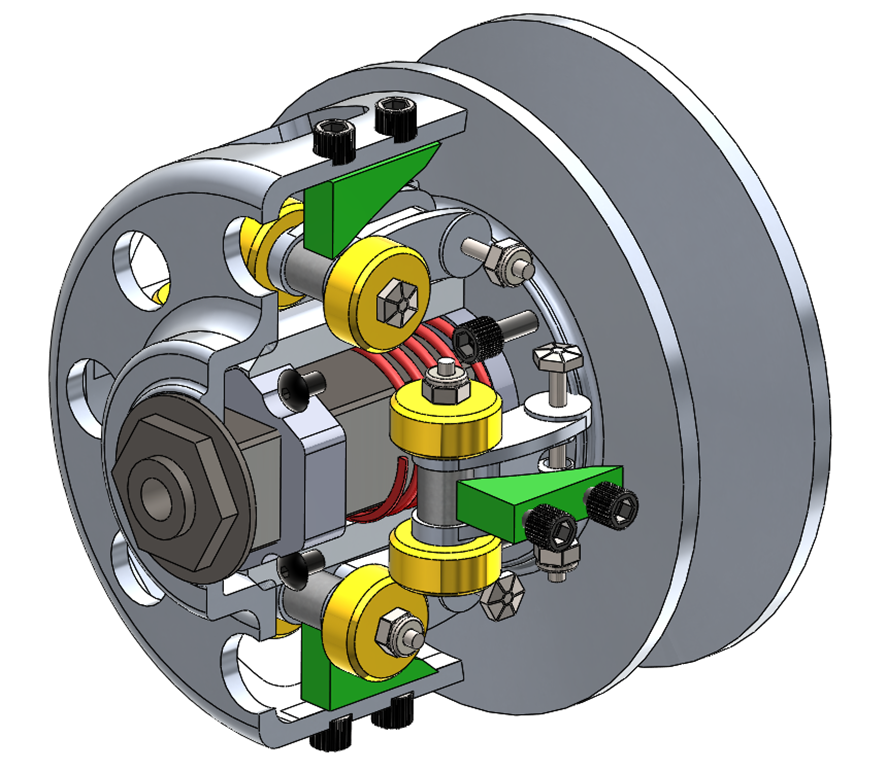
\includegraphics[scale=0.5]{primaryCVT.png}
          \caption{Primary CVT}
          \label{Fig_PrimaryCVT}
      \end{minipage}
      \hfill % This adds space between the figures
      \begin{minipage}{0.45\textwidth}
          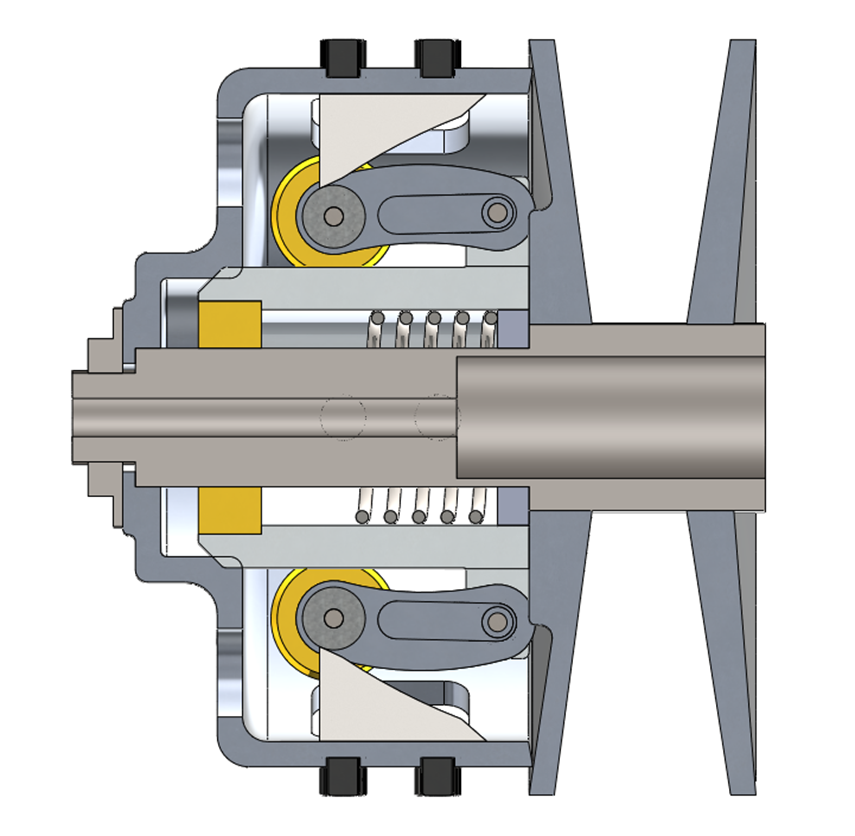
\includegraphics[scale=0.5]{primaryCVTSideView.png}
          \caption{Primary CVT Side View}
          \label{Fig_PrimaryCVTSideView}
      \end{minipage}
  \end{center}
\end{figure}

\begin{figure}[H]
  \begin{center}
      \begin{minipage}{0.45\textwidth}
          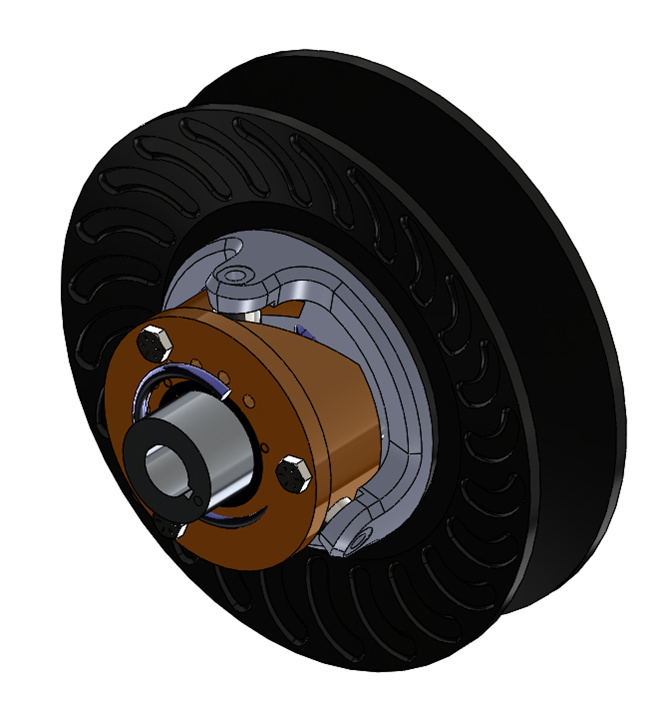
\includegraphics[scale=0.5]{secondaryCVT.png}
          \caption{Secondary CVT}
          \label{Fig_SecondaryCVT}
      \end{minipage}
      \hfill % This adds space between the figures
      \begin{minipage}{0.45\textwidth}
          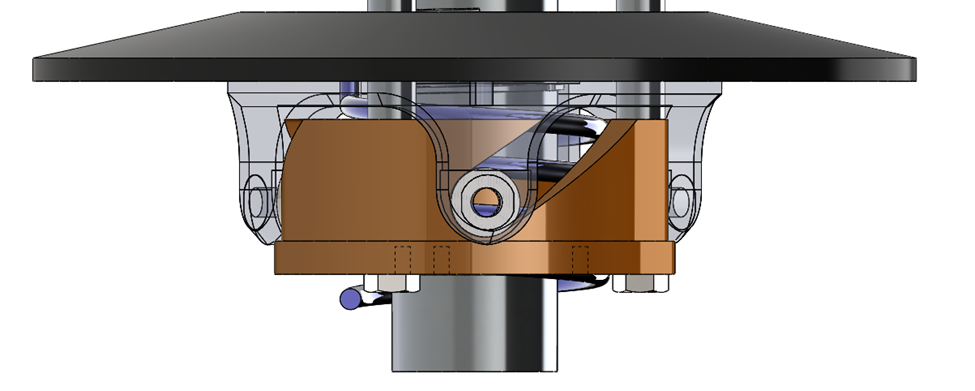
\includegraphics[scale=0.5]{secondaryCVTSideView.png}
          \caption{Secondary CVT Side View}
          \label{Fig_SecondaryCVTSideView}
      \end{minipage}
  \end{center}
\end{figure}

Note: While the McMaster Baja Team's CVT differs slightly from these figures, its mechanics remain widely equivalent.


\subsubsection{Physical System Description} \label{sec_phySystDescrip}

The physical system of \progname{}, as shown in Figures 2-5,
includes the following elements:

\begin{itemize}

\item[PS1:] Flyweights
\begin{itemize}
  \item [PS1a:] mass ($m_{\text{fly}}$) in kg.
  \item [PS1b:] initial radius ($r_{\text{fly}}$) in m.
\end{itemize}

\item[PS2:] Primary spring

\begin{itemize}
  \item [PS2a:] spring constant ($k_{\text{prim}}$) in N/m.
  \item [PS2b:] pre-compression distance ($d_{\text{prim}}$) in m.
\end{itemize}

\item[PS3:] Primary ramp geometry function ($f_{\text{prim\_angle}}$)

\begin{itemize}
  \item [PS3a:] shift distance ($d_{\text{shift}}$) in m.
  \item [PS3b:] output angle ($\theta_{\text{prim}}$) in radians.
\end{itemize}

\item[PS4:] Primary ramp height function ($f_{\text{prim\_height}}$)

\begin{itemize}
  \item [PS4a:] shift distance ($d_{\text{shift}}$) in m.
  \item [PS4b:] output height ($h_{\text{prim}}$) in m.
\end{itemize}

\item[PS5:] Secondary spring

\begin{itemize}
  \item [PS5a:] compression spring constant ($k_{\text{sec\_comp}}$) in N/m.
  \item [PS5b:] torsional spring rate ($k_{\text{sec\_tor}}$) in Nm/rad.
  \item [PS5c:] pre-compression distance ($d_{\text{sec}}$) in m.
  \item [P55d:] pre-torsional rotation ($\theta_{\text{sec}}$) in radians.
\end{itemize}

\item[PS6:] Secondary ramp geometry function ($f_{\text{sec\_ramp}}$)

\begin{itemize}
  \item [PS6a:] shift distance ($d_{\text{shift}}$) in m.
  \item [PS6b:] output angle ($\theta_{\text{ramp}}$) in radians.
\end{itemize}

\item[PS7:] Secondary ramp rotation function ($f_{\text{sec\_shift}}$)

\begin{itemize}
  \item [PS7a:] shift distance ($d_{\text{shift}}$) in m.
  \item [PS7b:] output angle ($\theta_{\text{shift}}$) in radians.
\end{itemize}

\item[PS8:] Weight

\begin{itemize}
  \item [PS8a:] driver weight ($m_{\text{d}}$) in kg.
  \item [PS8b:] vehicle weight ($m_{\text{v}}$) in kg.
\end{itemize}

\item[PS9:] Engine torque function ($f_{\text{engine}}$)

\begin{itemize}
  \item [PS9a:] input angular velocity ($\omega_{\text{engine}}$) in rad/s.
  \item [PS9b:] output torque ($T_{\text{eng}}$) in Nm.
\end{itemize}

\item[PS10:] Belt

\begin{itemize}
  \item [PS18a:] belt length ($l_{\text{belt}}$) in m.
  \item [PS18b:] belt width ($w_{\text{belt}}$) in m.
  \item [PS18c:] belt height ($h_{\text{belt}}$) in m.
  \item [PS18d:] belt weight ($m_{\text{belt}}$) in kg.
  \item [PS10b:] friction coefficient ($\mu_{\text{belt}}$), unitless.
\end{itemize}

\item[PS11:] Total reduction

\begin{itemize}
  \item [PS11a:] gearbox reduction ratio ($R_{\text{gearbox}}$), unitless.
  \item [PS11b:] wheel radius ($r_{\text{wheel}}$) in m.
\end{itemize}

\item[PS12:] Coefficient of air resistance ($\mu_{\text{air}}$), unitless.

\item[PS13:] Center to Center distance ($d_{\text{center}}$) in m.

\item[PS14:] Angle on Incline ($\theta_{\text{inc}}$) in radians.

\item[PS15:] Secondary Ramp Radius ($r_{\text{sec\_ramp}}$) in m.

\item[PS16:] Traction ($\mu_{\text{traction}}$), unitless.

\item[PS16:] CVT Geometry
\item[] \begin{itemize}
  \item [PS16a:] Primary shaft initial radius ($r_{\text{prim\_shaft}}$) in m.
  \item [PS16b:] Secondary shaft initial radius ($r_{\text{sec\_shaft}}$) in m.
\end{itemize}

\item[PS17:] Angle between sheaves ($\phi_{\text{sheave}}$) in radians. 

\end{itemize}

\subsubsection{Goal Statements}

\begin{itemize}

  \item[GS\refstepcounter{goalnum}\thegoalnum \label{GS1}:]  Given the material properties, initial conditions, and boundary conditions, predict the kinematics of the vehicle as a function of time, including its position, velocity, acceleration, and orientation.
  \item[GS\refstepcounter{goalnum}\thegoalnum \label{GS2}:]  Given the engine characteristics, load torque and time simulate the output of the engine as a function of time, predicting engine torque and angular velocity.
  \item[GS\refstepcounter{goalnum}\thegoalnum \label{GS3}:]  Given the flyweight specifications, spring coefficients, torque, input parameters, material properties, simulate the Continuous Variable Transmission (CVT) system over time, predict the output such as clamping forces, sheave acceleration, belt acceleration and system response to varying loads and engine outputs.

\end{itemize}

\subsection{Solution Characteristics Specification}
\begin{figure}[H]
  \includegraphics[scale=0.9]{RelationsBetweenTM_GD_IM_DD_A.pdf}
\end{figure}

The instance models that govern \progname{} are presented in
Subsection~\ref{sec_instance}.  The information to understand the meaning of the
instance models and their derivation is also presented, so that the instance
models can be verified.

\subsubsection{Types}

N/A

\subsubsection{Scope Decisions}

N/A
\subsubsection{Modelling Decisions}

N/A

\subsubsection{Assumptions} \label{sec_assumpt}

\begin{itemize}

\item[A\refstepcounter{assumpnum}\theassumpnum \label{A_1}:]
\textbf{No Material Variations By Temperature } Ignore the effect of temperature on the material properties, excluding the belt.

\item[A\refstepcounter{assumpnum}\theassumpnum \label{A_2}:]
\textbf{Negligible Gravitational Influence}: The orientation of the CVT system and gravitational effects are considered negligible due to the high rotational speeds involved in the system's operation.

\item[A\refstepcounter{assumpnum}\theassumpnum \label{A_3}:]
\textbf{Rigidity of Belts}: Elasticity of belts are assumed negligible through its length, and the components are considered ideally rigid under normal operating conditions. The belt may still rotate about the pulleys.

\item[A\refstepcounter{assumpnum}\theassumpnum \label{A_4}:]
\textbf{No Vibrational Effects}: Vibrational effects from the vehicle or external environment are assumed to be minimal and are not factored into the transmission’s operation in this model.

\item[A\refstepcounter{assumpnum}\theassumpnum \label{A_5}:]
\textbf{Ignore Wear and Tear}: Component wear over time, including belt/chain wear and pulley degradation, is assumed negligible in the short-term operational model.

\item[A\refstepcounter{assumpnum}\theassumpnum \label{A_6}:]
\textbf{No Frictional Losses in Non-critical Components}: Frictional losses in non-critical components (e.g., bearings, shafts) are assumed negligible, focusing only on friction relevant to the CVT system's core mechanics.

\item[A\refstepcounter{assumpnum}\theassumpnum \label{A_7}:]
\textbf{Full Throttle Consistent Power Engine:} The engine is modeled to operate at full throttle with consistent power curves and peak performance, maintaining a uniform response throughout the analysis. Load feedback will be integrated to adjust RPM and power output as necessary.

\item[A\refstepcounter{assumpnum}\theassumpnum \label{A_8}:]
\textbf{Perfect Axis Alignment:} The CVT's axes are aligned with one another.

\item[A\refstepcounter{assumpnum}\theassumpnum \label{A_9}:]
\textbf{No Belt Slippage:} The CVT will not slip relative to the sheaves.

\item[A\refstepcounter{assumpnum}\theassumpnum \label{A_10}:]
\textbf{Ignore Irrelevant Forces:} Only forces that directly contribute to the car's dynamics or the CVT's shifting behaviours are considered, allowing the simplification of dimensions where applicable.

\end{itemize}

\subsubsection{Theoretical Models}\label{sec_theoretical}

This section focuses on the general equations and laws that \progname{} is based
on. 
\subsubsection*{General Theories}
This portion will specify the existing theories that are used in the development of the CVT simulation tool.

\noindent
\deftheory
{TM:HL}% #2 refname of theory
{Hookes Law (Displacement)}% #3 label
{$F = k \Delta x$}% #4 equation
{$F$ is the force (N)\\
  $k$ is the spring constant (N/m)\\
  $\Delta x$ is the displacement (m)}% #5 description
{In the context of this project Hookes law is used in both a torsional and linear way.}% #6 Notes
{\url{https://www.britannica.com/science/Hookes-law}}% #7 Source
{IM\ref{inst:4}}% #8 Referenced by
{None}% #9 Preconditions
{}% #1 derivation - not applicable by default

~\newline

\noindent
\deftheory
{TM:CF}% #2 refname of theory
{Centrifugal Force}% #3 label
{$F_c = m \omega^2 r$}% #4 equation
{$F$ is the force (N) \\
  $m$ is the mass (kg)\\
  $\omega$ is the angular velocity (rad/s)\\
  $r$ is the radius (m)}% #5 description
{None.}% #6 Notes
{\url{https://www.omnicalculator.com/physics/centrifugal-force}}% #7 Source
{IM\ref{inst:4}}% #8 Referenced by
{None}% #9 Preconditions
{}% #1 derivation - not applicable by default

~\newline

\noindent
\deftheory
{TM:AR}% #2 refname of theory
{Air Resistance}% #3 label
{$F_d = \frac{1}{2} \rho v^2 C_d A$}% #4 equation
{F is the force (N)\\
  $\rho$ is the density of the fluid (kg/m$^3$)\\
  $v$ is the velocity of the object (m/s)\\
  $C_d$ is the drag coefficient\\
  $A$ is the cross-sectional area of the object (m$^2$)}% #5 description
{None.}% #6 Notes
{\url{https://softschools.com/formulas/physics/air_resistance_formula/85/}}% #7 Source
{IM\ref{inst:1}}% #8 Referenced by
{None}% #9 Preconditions
{}% #1 derivation - not applicable by default

~\newline

\noindent
\deftheory
{TM:ET} % #2 refname of theory
{Engine Torque} % #3 label
{$\tau = \frac{P}{\omega}$} % #4 equation
{$\tau$ is the torque (Nm)\\
  $P$ is the power (W)\\
  $\omega$ is the angular velocity (rad/s)}% #5 description
{None.}% #6 Notes
{\url{https://powertestdyno.com/how-to-calculate-horsepower/}}% #7 Source
{}% #8 Referenced by
{None}% #9 Preconditions
{}% #1 derivation - not applicable by default

~\newline

\noindent
\deftheory
{TM:GR}% #2 refname of theory
{Gearing}% #3 label
{$\tau_{\text{output}} = \tau_{\text{input}} \times R_\text{gear}$}% #4 equation
{$\tau_{\text{output}}$ is the output torque (Nm)\\
  $\tau_{\text{input}}$ is the input torque (Nm)\\
  $R_\text{gear}$ is the gear reduction (unitless)}% #5 description
{None.}% #6 Notes
{\url{https://science.howstuffworks.com/transport/engines-equipment/gear-ratio.htm}}% #7 Source
{IM\ref{inst:1}}% #8 Referenced by
{None}% #9 Preconditions
{}% #1 derivation - not applicable by default

~\newline

\noindent
\deftheory
{TM:FR}% #2 refname of theory
{Static Friction Formula}% #3 label
{$F_f = \mu_s F_n$}% #4 equation
{$\mu_s$ is the coefficient of friction (unitless)\\
  $F_f$ is the force of friction (N)\\
  $F_n$ is the normal force (N)}% #5 description
{None.}% #6 Notes
{\url{https://en.wikipedia.org/wiki/Friction}}% #7 Source
{IM\ref{inst:1}, IM\ref{inst:7}}% #8 Referenced by
{None}% #9 Preconditions
{}% #1 derivation - not applicable by default

\noindent
\deftheory
{TM:DE}% #2 refname of theory
{Density}% #3 label
{$\rho = \frac{m}{V}$}% #4 equation
{$\rho$ is the density (kg/m$^3$)\\
  $m$ is the mass (kg)\\
  $V$ is the volume (m$^3$)}% #5 description
{None.}% #6 Notes
{\url{https://www.britannica.com/science/density-physics}}% #7 Source
{IM\ref{inst:1}}% #8 Referenced by
{None}% #9 Preconditions
{}% #1 derivation - not applicable by default

~\newline

\noindent
\deftheory
{TM:CE}% #2 refname of theory
{Capstan Equation}% #3 label
{$T_1 = T_2 e^{\mu \theta}$}% #4 equation
{$T_1$ is the tension on the first side of the belt (N)\\
  $T_2$ is the tension on the second side of the belt (N)\\
  $\mu$ is the coefficient of friction\\
  $\theta$ is the angle of wrap of the belt (radians)}% #5 description
{None.}% #6 Notes
{\url{https://hackaday.com/2021/01/26/cable-mechanism-maths-designing-against-the-capstan-equation/}}% #7 Source
{IM\ref{inst:7}}% #8 Referenced by
{None}% #9 Preconditions
{}% #1 derivation - not applicable by default

~\newline

\noindent
\deftheory
{TM:N2}% #2 refname of theory
{Newtons 2nd Law}% #3 label
{$F = ma$}% #4 equation
{  $F$ is the force (N)\\
  $m$ is the mass (kg)\\
  $a$ is the acceleration (m/s$^2$)}% #5 description
{Newtons 2nd law is used repeatedly in several Instance models}% #6 Notes
{\url{https://www.physicsclassroom.com/class/newtlaws/lesson-3/newton-s-second-law}}% #7 Source
{IM\ref{inst:1}, IM\ref{inst:6}, IM\ref{inst:7}}% #8 Referenced by
{None}% #9 Preconditions
{}% #1 derivation - not applicable by default

\subsubsection*{Helper Theories}
This portion will define auxiliary theories to aid in further derivation below.

\noindent
\deftheory
{TM:D2R}% #2 refname of theory
{Shift Distance to Pulley Radius}% #3 label
{$\Delta r = \frac{d_\text{shift}}{2\tan(\frac{\phi}{2})}$}% #4 equation
{$d_\text{shift}$ is the axial shift distance, or sheave displacement (m)\\
$\Delta r$ is the change in effective radius (m)\\
$\phi$ is the angle between sheaves (rad)}% #5 description
{Derived based on geometry of the sheaves and belt}% #6 Notes
{See below for derivation}% #7 Source
{}% #8 Referenced by
{None}% #9 Preconditions
{}% #1 derivation - not applicable by default

\noindent
\deftheory
{TM:D2RA}% #2 refname of theory
{Shift Distance to Ramp Angle}% #3 label
{$\theta_\text{ramp} = f_\text{prim}(d_\text{shift})$}% #4 equation
{$d_\text{shift}$ is the axial shift distance, or sheave displacement (m)\\
$\theta_\text{ramp}$ is the instantaneous ramp angle (rad)\\
$f_\text{prim}(d)$ is the function to express the ramp geometry (m $\rightarrow$ rad)}% #5 description
{The user will input the geometry of the ramp, which will then be intepreted to generate $f_\text{prim}$}% #6 Notes
{See below for derivation}% #7 Source
{}% #8 Referenced by
{None}% #9 Preconditions
{}% #1 derivation - not applicable by default

\noindent
\deftheory
{TM:D2HA}% #2 refname of theory
{Shift Distance to Helix Angle}% #3 label
{$\theta_\text{ramp} = f_\text{sec}(d_\text{shift})$}% #4 equation
{$d_\text{shift}$ is the axial shift distance, or sheave displacement (m)\\
$\theta_\text{ramp}$ is the instantaneous helix angle (rad)\\
$f_\text{prim}(d)$ is the function to express the helix geometry (m $\rightarrow$ rad)}% #5 description
{The user will input the geometry of the helix, which will then be intepreted to generate $f_\text{sec}$}% #6 Notes
{See below for derivation}% #7 Source
{}% #8 Referenced by
{None}% #9 Preconditions
{}% #1 derivation - not applicable by default

\noindent
\deftheory
{TM:HT}% #2 refname of theory
{Hookes Law (Torsional)}% #3 label
{$F = \frac{k \Delta \theta}{r} $}% #4 equation
{$F$ is the force (N)\\
  $k$ is the torsional spring constant (Nm/rad)\\
  $\Delta \theta$ is the rotation (rad)
  $r$ is the radius of the applied torque (m)
  }% #5 description
{}% #6 Notes
{\url{https://www.drtempleman.com/spring-resources-old/spring-design-formulas-2}}% #7 Source
{}% #8 Referenced by
{None}% #9 Preconditions
{}% #1 derivation - not applicable by default

\noindent
\deftheory
{TM:KE}% #2 refname of theory
{Kinetic Energy}% #3 label
{$KE = \frac{1}{2} m v^2$}% #4 equation
{$KE$ is the kinetic energy (J)\\
  $m$ is the mass (kg)\\
  $v$ is the velocity (m/s)
}% #5 description
{None.}% #6 Notes
{\url{https://www.physicsclassroom.com/class/energy/Lesson-1/Kinetic-Energy}}% #7 Source
{}% #8 Referenced by
{None}% #9 Preconditions
{}% #1 derivation - not applicable by default

~\newline

\subsubsection{General Definitions}\label{sec_gendef}

\defgeneral
{Helix Side Force} % #1 label
{N = \si{\kilogram \metre\per\square\second}} % #2 units
{$F_H = \frac{T_\text{eng} R_\text{cvt}}{2r\tan(\beta)}$} % #3 equation
{$F_H$ is the side force due to the helix (N) \\
& $T_{\text{eng}}$ is the engine torque (N-m) \\
& $R_{\text{CVT}}$ is the CVT ratio (unitless) \\
& $r$ is the radius of the ramps from the shaft (m) \\
& $\beta$ is the helix angle (rad)} % #4 description
{} % #5 source
{\iref{inst:5}} % #6 referenced by

\subsubsection*{Derivation of Helix Side Force}
The helix side force can be derived from using the torque across the CVT system, then by dividing out the radius to get a force.

\[ T_\text{CVT} = T_\text{eng} \cdot R_\text{cvt} \tag*{\text{(see \hyperref[TM:GR]{TM:GR})}}\]

Since this is a torque, we can convert it to a force by dividing by the radius of the ramps. Further, since the ramps are angled at $\beta$, we divide by $\tan(\beta)$ to get the force in the direction of the helix (see \aref{A_10}). Finally, since only one of the two pulleys is moveable, and the force is acting on both, we must divide by a factor of 2.

\[ F_H = \frac{T_\text{eng} R_\text{cvt}}{2r\tan(\beta)} \]


\defgeneral
{Spring Side Force} % #1 label
{N = \si{\kilogram \metre\per\square\second}} % #2 units
{\[F_S = \frac{k_{\text{tor}}(\theta_0 + \theta)}{2r\tan(\beta)} + k_\text{comp}(x_0 + x)\]} % #3 equation
{$F_S$ is the side force due to the spring (N) \\
& $k_{\text{tor}}$ is the torsional spring constant (\si[per-mode=symbol] {\newton\metre\per\radian}) \\
& $\theta_0$ is the initial torsion (rad) \\
& $\theta$ is the amount of angular torsion (rad) \\
& $k_{\text{comp}}$ is the compression spring constant (\si[per-mode=symbol] {\newton\per\metre}) \\
& $x_0$ is the initial compression (m) \\
& $x$ is the amount of compression (m) \\
& $r$ is the radius of the ramps from the shaft (m) \\
& $\theta$ is the amount of angular torsion (rad)} % #4 description
{} % #5 source
{\iref{inst:5}} % #6 referenced by

\subsubsection*{Derivation of Spring Side Force}

This portion of the secondary side force can be split into two components, the torsional spring force and the compression spring force. 
Beginning with the compression spring force, we can use \hyperref[TM:HL]{Hooke's Law} to derive:

\[ F_{\text{comp}} = k_{\text{comp}} \cdot x \tag*{\text{(see \hyperref[TM:HL]{TM:HL})}}\]

Here, the displacement $x$ is the change in the compression of the spring added with the precompression based on the tune.

\[ F_{\text{comp}} = k_{\text{comp}} \cdot (x_0 + x) \tag*{\text{(see \hyperref[TM:HL]{TM:HL})}}\]

Next, we can derive the torsional spring force. We can use \hyperref[TM:HT]{Hooke's Law (Torsional)} to derive:

\[ T_{\text{tor}} = \frac{k_{\text{tor}} \cdot \theta}{r} \tag*{\text{(see \hyperref[TM:HT]{TM:HT})}}\]

Similarily, we have an initial torsional compression $\theta_0$ that is added to the current torsional compression $\theta$.

\[ F_{\text{tor}} = \frac{k_{\text{tor}} \cdot (\theta_0 + \theta)}{r} \]

Since this force is acting against the helix's angle, we must divide by $\tan(\beta)$ to get the force in the direction of the helix. Finally, since only one of the two pulleys is moveable, and the force is acting on both, we must divide by a factor of 2.

\[ F_S = \frac{k_{\text{tor}}(\theta_0 + \theta)}{2r\tan(\beta)} + k_\text{comp}(x_0 + x) \]

Combining the two forces, we get the total side force acting on the secondary CVT created by the spring.

\[ F_S = \frac{k_{\text{tor}}(\theta_0 + \theta)}{2r\tan(\beta)} + k_\text{comp}(x_0 + x) \]


% TODO: Add derivation

\subsubsection{Data Definitions}\label{sec_datadef}

This section collects and defines all the data needed to build the instance
models. The dimension of each quantity is also given. 

\defdata 
{Friction}% #1 refname of data
{Coefficient of Friction} % #2 label
{$\mu$} % #3 symbol
{unitless} % #4 units
{$F_f = \mu F_n$} % #5 equation
{$\mu$ is the coefficient of friction\\
& $F_f$ is the force of friction\\
& $F_n$ is the normal force}% #6 description
{None.}% #7 Source
{IM\ref{inst:1}, IM\ref{inst:7}}% #8 Referenced by

\defdata 
{SpringConstComp}% #1 refname of data
{Compressionional Spring Constant} % #2 label
{$k$} % #3 symbol
{\si[per-mode=symbol] {\newton\per\metre}} % #4 units
{$F = k \Delta x$} % #5 equation
{$k$ is the spring constant (\si[per-mode=symbol] {\newton\per\metre})\\
& $F$ is the force (\si[per-mode=symbol] {\newton})\\
& $\Delta x$ is the displacement (\si[per-mode=symbol] {\metre})}% #6 description
{None.}% #7 Source
{IM\ref{inst:4}}% #8 Referenced by

\defdata
{SpringConstTors}% #1 refname of data
{Torsional Spring Constant} % #2 label
{$k$} % #3 symbol
{\si[per-mode=symbol] {\newton\metre\per\radian}} % #4 units
{$\tau = k \Delta \theta$} % #5 equation
{$k$ is the torsional spring constant (\si[per-mode=symbol] {\newton\metre\per\radian})\\
& $\tau$ is the torque (\si[per-mode=symbol] {\newton\metre})\\
& $\theta$ is the angle of rotation (radians)} % #6 description
{None.}% #7 Source
{IM\ref{inst:5}}% #8 Referenced by

\defdata 
{GravConst}
{Gravitational Constant}
{$g$}
{\si[per-mode=symbol] {\metre\per\square\second}}
{$F_g = m g$}
{$g$ is the gravitational constant (\si[per-mode=symbol] {\metre\per\square\second})\\
& $F_g$ is the force of gravity\\
& $m$ is the mass}% #6 description
{None.}% #7 Source
{IM\ref{inst:1}}% #8 Referenced by

\defdata 
{DragCoeff}
{Drag Coefficient}
{$C_d$}
{unitless}
{$F_d = \frac{1}{2} \rho v^2 C_d A$}
{$C_d$ is the drag coefficient\\
& $F_d$ is the force of drag\\
& $\rho$ is the density of the fluid\\
& $v$ is the velocity of the object\\
& $A$ is the cross-sectional area of the object}% #6 description
{None.}% #7 Source
{IM\ref{inst:1}}% #8 Referenced by

\defdata 
{RollCoeff}
{Rolling Resistance Coefficient}
{$C_{\text{rr}}$}
{unitless}
{$F_{\text{rr}} = C_{\text{rr}} F_n$}
{$C_{\text{rr}}$ is the rolling resistance coefficient\\
& $F_{\text{rr}}$ is the force of rolling resistance\\
& $F_n$ is the normal force}% #6 description
{None.}% #7 Source
{IM\ref{inst:1}}% #8 Referenced by

\subsubsection{Data Types}\label{sec_datatypes}

N/A

\subsubsection{Instance Models} \label{sec_instance}    

This section transforms the problem defined in Section~\ref{Sec_pd} into 
one which is expressed in mathematical terms. It uses concrete symbols defined 
in Section~\ref{sec_datadef} to replace the abstract symbols in the models 
identified in Sections~\ref{sec_theoretical} and~\ref{sec_gendef}.
{\newline}

{\noindent}The goal statment GS\ref{GS1} are solved by Instance Models \ref{inst:1}, \ref{inst:2} and \ref{inst:3}\\
{\noindent}The goal statement GS\ref{GS2} are solved by Instance Models \ref{inst:8}\\
The goal statement GS\ref{GS3} are solved by Instance Models \ref{inst:4}, \ref{inst:5}, \ref{inst:6} and \ref{inst:7}\\
  \definstance
  {Acceleration}
  {$r_{\text{gear}}, r_{\text{wheel}}, \rho, C_d, A, \theta_{\text{inc}}, T_{\text{CVT}}, C_{\text{rr}}, m_v, m_d$}
  {
    \[ a(t) = \frac{\left( \frac{T_{\text{eng}}(t) \cdot R_\text{cvt}(t)}{r_{\text{gear}} + r_{\text{wheel}}} \right) - (C_{\text{rr}} F_g \sin(\theta_\text{inc})) - \left( \frac{1}{2} \rho v^2 C_D A \right) - (F_g \cos(\theta_\text{inc}))}{m_v + m_d} \]
    }
  {acceleration $a(t)$}
  {
  $r_{\text{gear}}$ is the radius of the gear (m)\\
  & $r_{\text{wheel}}$ is the radius of the wheel (m)\\
  & $\rho$ is the density of the fluid (kg/m$^3$)\\
  & $C_d$ is the drag coefficient (unitless)\\
  & $A$ is the cross-sectional area of the object (m$^2$)\\
  & $\theta_{inc}$ is the angle of incline (rad)\\
  & $C_{\text{rr}}$ is the coefficient of rolling resistance (unitless)\\
  & $F_g$ is the force of gravity (N)\\
  & $m_v$ is the mass of the vehicle (kg)\\
  & $m_d$ is the mass of the driver(kg)\\
  & $a(t)$ is the function of acceleration over time (m/s$^2$)\\
  & $R_\text{cvt}(t)$ is the current ratio of the CVT as a function of time (unitless)\\
  & $T_{\text{eng}}(t)$ is the torque seen at the engine as a function of time (Nm)
}
  {\iref{inst:5}}
  {-}
  
  
  \subsubsection*{Derivation of Acceleration}

Using \hyperref[TM:N2]{Newton's 2nd Law}, the acceleration of the vehicle is derived as follows: 
\[
T_W - R_r - F_D - F_g \cos(\theta_\text{inc}) = ma
\]
Where \( T_W \) is the torque of the wheel, \( F_r \) is the rolling resistance, \( F_D \) is the drag force, \( F_g \) is the gravitational force, and \( m \) is the mass of the vehicle. 

\[
T_W = \frac{T_{\text{eng}}(t) \cdot R_\text{cvt}(t)}{r_{\text{gear}} + r_{\text{wheel}}} \tag*{\text{(see \hyperref[TM:GR]{TM:GR})}}
\],

\[
F_r = C_{\text{rr}} F_g \sin(\theta_{inc}) \tag*{\text{(see \hyperref[TM:FR]{TM:FR})}}
\]

\[
F_D = \frac{1}{2} \rho v^2 C_D A \tag*{\text{(see \hyperref[TM:AR]{TM:AR})}}
\]

\[
m = m_v + m_d
\]

Substituting the above equations in and solving for $a$ gives us the final equation:
\[ a(t) = \frac{\left( \frac{T_{\text{eng}}(t) \cdot R_\text{cvt}(t)}{r_{\text{gear}} + r_{\text{wheel}}} \right) - (C_{\text{rr}} F_g \sin(\theta_\text{inc})) - \left( \frac{1}{2} \rho v^2 C_D A \right) - (F_g \cos(\theta))}{m_v + m_d} \]
\definstance
{Velocity}
{$a(t)$}
{$v(t) = \int a(t) dt$}
{$v(t)$}
{$a(t)$ is the function of acceleration over time}
{-}

\definstance
{Distance}
{$v(t)$}
{$d(t) = \int v(t) dt$}
{$d(t)$}
{$v(t)$ is the function of velocity over time}
{-}

\definstance
{Primary Clamping Force}
{$m_\text{fly}$, $r_{\text{fly}}$, $f_{\text{prim\_height}}(d_{\text{shift}})$, $f_{\text{prim\_angle}}(d_{\text{shift}}(t))$, $k_{\text{prim}}$, $d_{\text{prim}}$, $d_{\text{shift}}$} % Input
{$F_{\text{prim\_clamp}}(t) = m_\text{fly} (r_{\text{fly}} + f_{\text{prim\_height}}({d_\text{shift}(t)}))(\omega_\text{eng}(t))^2 \tan(f_{\text{prim\_angle}}(d_\text{shift}(t))) + k_{\text{prim}} (d_{\text{prim}} + d_\text{shift}(t))$} % 
{The primary clamping force $F_{\text{prim\_clamp}}$}
{$m_\text{fly}$: Mass of the flyweight system. (kg) \\ 
  &$r_{\text{fly}}$: Initial radius of the flyweights. (m) \\ 
  &$f_{\text{prim\_height}}(d_{\text{shift}})$: Function that represents the height of the flyweights based on the shift distance. (rad) \\
  &$f_{\text{prim\_angle}}(d_{\text{shift}})$: Function that returns the instantaneous angle of the ramps based on the shifting distance. (rad) \\ 
  &$k_{\text{prim}}$: Primary spring coefficient. (unitless) \\ 
  &$d_\text{shift}(t)$: Displacement of the sheave as a function of time. (m)\\
  &$\omega_\text{eng} (t)$: Angular velocity of the engine as a function of time. (rad/s)\\
  &$d_{\text{prim}}$: Initial compression distance of the primary spring. (m)
} % Description
{} % Sources
{\iref{inst:6}}

\subsubsection*{Derivation of Primary Clamping Force}

The flyweight experiences a \hyperref[TM:CF]{centrifugal force} {$F_c = m r\omega^2 $} as it rotates. 
The ramp angle $f_{\text{prim\_angle}}(d_{\text{shift}})$ is where the force applied by the flyweight meets the inclined surface.
The force can be broken into the radial force, which is perpendicular to the ramp, and the axial force which acts in the direction of the ramp.
The axial force is what is responsible for moving the mechanism causing the flyweights to press against a ramp or surface, therefore the force we are interested in.
We can ignore the radial force as it acts perpendicular to the ramp and does not contribute to the axial force. (see \aref{A_10})
To find the flywheel force in this axial direction the tangent of the angle $f_{\text{prim\_angle}}(d_{\text{shift}})$ is used.
The flywheel force is derived as follows: 
\[
F_{FW} = m r \omega^2 \tan(f_{\text{prim\_angle}}(d_{\text{shift}})) \tag*{\text{(see \hyperref[TM:CF]{TM:CF})}}
\]
Where \( r \) can be represented by \( r_{\text{fly}} + f_{\text{prim\_height}}(d_{\text{shift}}) \). Then \( F_{FW} \) becomes 
\[
F_{FW} = m_\text{fly} (r_{\text{fly}} + f_{\text{prim\_height}}(d_{\text{shift}}))\omega^2 \tan(f_{\text{prim\_angle}}(d_{\text{shift}}))
\]

The spring force is derived as follows: 
\[
-F_S = + k_{\text{prim}} (d_{\text{prim}} + d_{\text{shift}}) \tag*{\text{(see \hyperref[TM:HL]{TM:HL})}}
\]

Combining these two forces gives the total primary clamping force:
\[
F_{FW} - F_S =  m_\text{fly} (r_{\text{fly}} + f_{\text{prim\_height}}(d_{\text{shift}}))\omega^2 \tan(f_{\text{prim\_angle}}(d_{\text{shift}})) + k_{\text{prim}} (d_{\text{prim}} + d_{\text{shift}})
\]

The final equation can be written as:
\[
F_{\text{prim\_clamp}}(t) = m_\text{fly} (r_{\text{fly}} + f_{\text{prim\_height}}({d_\text{shift}(t)}))(\omega_\text{eng}(t))^2 \tan(f_{\text{prim\_angle}}(d_\text{shift}(t))) + k_{\text{prim}} (d_{\text{prim}} + d_\text{shift}(t))
\]

\definstance
{Secondary Clamping Force}
{$k_{\text{sec\_tor}}$, $\theta_{\text{sec}}$, $r_{\text{sec\_ramp}}$, $f_{\text{sec\_ramp}}(d_{\text{shift}})$, $f_{\text{sec\_shift}}(d_{\text{shift}})$, $k_{\text{sec\_comp}}$, $d_{\text{sec}}$, $d_{\text{shift}}(t)$, $T_{eng}(t)$, $R_{cvt}(t)$} % Input
{\[
F_{\text{sec\_clamp}}(t) = \frac{k_{\text{sec\_tor}} (\theta_{\text{sec}} + f_{\text{sec\_shift}}(d_\text{shift}(t))) + T_{eng}(t) R_{cvt}(t)}{2 r_{\text{sec\_ramp}} \tan(f_{\text{sec\_ramp}}(d_{\text{shift}}(t)))} + k_{\text{sec\_comp}} (d_{\text{sec}} + d_{\text{shift}}(t))
\]} % 
{Secondary clamping force $F_{\text{sec\_clamp}}$} % Output
{$k_{\text{sec\_tor}}$: Torsional spring rate. (Nm/rad)\\
  &$\theta_{\text{sec}}$: Initial torsional rotation. (rad)\\
  &$f_{\text{sec}}(d_{\text{shift}})$: Amount of torsional rotation based on the distance shifted. (rad) \\
  &$r_{\text{sec\_ramp}}$: Radius of the helix from the shaft. (m)\\
  &$k_{\text{sec\_comp}}$: Compression spring rate. (N/m)\\
  &$d_{\text{sec}}$: Initial compression distance. (m)\\
  &$d_{\text{shift}}$: Displacement of the sheave as a function of time. (m)\\
  &$T_{eng}(t)$: Torque seen at the engine as a function of time. (Nm) \\
  &$R_{cvt}(t)$: Ratio of the CVT as a function of time. (unitless)
} % Description
{} % Sources
{\iref{inst:6}}

\subsubsection*{Derivation of Secondary Clamping Force}

The secondary clamping force is derived as follows:
\[
F_{\text{sec\_clamp}}\ = F_H + F_S
\]

The helix force is derived as follows:

\[
F_H = \frac{T_{eng}(t) R_{cvt}(t)}{2r\tan(\beta)}  \tag*{\text{(see \dref{GD_2})}} % TODO: Fix reference
\]

Substituting in our variables gives us the following equation:

\[
F_H = \frac{T_{eng}(t) R_{cvt}(t)}{2 r_{\text{sec\_ramp}} \tan(f_{\text{sec\_ramp}}(d_\text{shift}(t)))}
\]

The spring force is derived as follows:

\[
F_S = \frac{k_{\text{tor}}(\theta_0 + \theta)}{2r\tan(\beta)} + k_\text{comp}(x_0 + x) \tag*{\text{(see \dref{GD_1})}} % TODO: Fix reference
\]

Substituting in our variables gives us the following equation:
\[
F_S = \frac{k_{\text{sec\_tor}} (\theta_{\text{sec}} + f_{\text{sec\_shift}}(d_\text{shift}(t)))}{2 r_{\text{sec\_ramp}} \tan(f_{\text{sec\_ramp}}(d_\text{shift}(t)))} + k_{\text{sec\_comp}} (d_{\text{sec}} + d_\text{shift}(t))
\]

Combining these two forces gives the total secondary clamping force:
\[
F_H + F_S = \frac{T_{eng}(t) R_{cvt}(t)}{2 r_{\text{sec\_ramp}} \tan(f_{\text{sec\_ramp}}(d_\text{shift}(t)))} + \frac{k_{\text{sec\_tor}} (\theta_{\text{sec}} + f_{\text{sec\_shift}}(d_\text{shift}(t)))}{2 r_{\text{sec\_ramp}} \tan(f_{\text{sec\_ramp}}(d_\text{shift}(t)))} + k_{\text{sec\_comp}} (d_{\text{sec}} + d_\text{shift}(t))
\]

The final equation can be reached through simplifying the above equation by combining like terms:
\[
F_{\text{sec\_clamp}} = \frac{k_{\text{sec\_tor}} (\theta_{\text{sec}} + f_{\text{sec\_shift}}(d_\text{shift}(t))) + T_{eng}(t) R_{cvt}(t)}{2 r_{\text{sec\_ramp}} \tan(f_{\text{sec\_ramp}}(d_\text{shift}(t)))} + k_{\text{sec\_comp}} (d_{\text{sec}} + d_\text{shift}(t))
\]

% TODO: Clean up T_T and T_s, shouldnt's exist like this? These are forces that change over time, its why we derived them below
\definstance
{Sheave Acceleration}
{$F_{\text{clamp\_prim}}, F_{\text{clamp\_sec}}, m_\text{sheaves}$} % Input
{\[a(t) = \frac{F_{\text{clamp\_prim}}(t) - F_{\text{clamp\_sec}}(t)}{m_\text{sheaves}}\]} % Equation
{Sheave acceleration $a$} % Output
{$F_{\text{clamp\_prim}}$: Primary clamping force\\
  &$F_{\text{clamp\_sec}}$: Secondary clamping force\\
  &$m_\text{sheaves}$: Mass of the movable sheaves, combined} % Description
{} % Sources
{-}
{} % Sources
{} % Citation
{-}

\subsubsection*{Derivation of Sheave Acceleration}
One can derive the accleration of the sheaves using \hyperref[TM:N2]{Newton's Second Law}. The forces acting on the built include 
only the primary and secondary clamping forces, which act in opposite directions as they act out radially.
The acceleration of the sheave is derived as follows:
\[ma(t) = F_{\text{clamp\_prim}}(t) - F_{\text{clamp\_sec}}(t)\]
Rearranging the equation for acceleration gives the final equation:
\[a(t) = \frac{F_{\text{clamp\_prim}}(t) - F_{\text{clamp\_sec}}(t)}{m}\]



\definstance
{Belt Acceleration}
{$T_{\text{eng}}, r_{\text{prim}}, m_\text{belt}$ } % Input
{$a_{\text{belt}} = \frac{T_{\text{eng}}}{m r_{\text{prim}}}$} % Equation
{Belt Acceleration $a_{\text{belt}}$} % Output
{$T_{\text{eng}}$: Engine torque\\
   &$r_{\text{prim}}$: Primary radiu\\
   &$m_\text{belt}$: Mass of the belt.} % Description} % Description
{} % Sources
{IM6} % Citation
\subsubsection*{Derivation of Belt Acceleration}

The torque of the engine equation in terms of belt tension is derived as such: \\
\[T_{\text{eng}} = (T_T - T_s) r_{\text{prim}} \quad \Rightarrow \quad T_T - T_s = \frac{T_{\text{eng}}}{r_{\text{prim}}}\] % TODO: Add TM and reference here
Similarly, for the load torque: \\
\[T_{\text{load}} = (T_T - T_s) r_{\text{sec}} \quad \Rightarrow \quad T_T - T_s = \frac{T_{\text{load}}}{r_{\text{sec}}}\] % TODO: Add TM and reference here
Equating the two torque equations: \\
\[\frac{T_{\text{eng}}}{r_{\text{prim}}} = \frac{T_{\text{load}}}{r_{\text{sec}}} \tag*{\text{(see \aref{A_9})}}\] 
{\newline}

The equation for the torque of the taut side is derived using the \hyperref[TM:CE]{capstan equation}:
\[T_T = T_s e^{\mu \theta} \tag*{\text{(\hyperref[TM:CE]{TM:CE})}}\]
Substituting our engine torque into this: \\
\[\frac{T_{\text{eng}}}{r_{\text{prim}}} + T_s = T_s e^{\mu \theta}\]
Solving for \(T_s\) (slack side): \\
\[T_s = \frac{T_{\text{eng}}}{r_{\text{prim}} (e^{\mu \theta} - 1)}\]
{\newline}

Using \hyperref[TM:N2]{Newton's 2nd law} the final equation for belt acceleration is derived as: \\
\[m_\text{belt} a_{\text{belt}} = \frac{T_{\text{eng}} e^{\mu \theta}}{r_{\text{prim}} (e^{\mu \theta} - 1)} - \frac{T_{\text{eng}}}{r_{\text{prim}} (e^{\mu \theta} - 1)}  \tag*{\text{(\hyperref[TM:N2]{TM:N2})}}\]
Solving for acceleration: \\
\[a_{\text{belt}} = \frac{T_{\text{eng}}}{m_\text{belt} r_{\text{prim}} (e^{\mu \theta} - 1)} (e^{\mu \theta} - 1)\]
Finally, simplifying to get: \\
\[a_{\text{belt}} = \frac{T_{\text{eng}}}{m_\text{belt} r_{\text{prim}}}\]


% TODO: Probably need to define this if I can't find a source
\definstance
{RPM and Torque of Engine}
{$t, T_\text{load}$} % Input
{{$T_{eng}$,  $\omega_\text{eng}$ } = $F(t, T_\text{load})$} % Equation
{$T_{eng}$, $\omega_\text{eng}$} % Output
{
  $T_{eng}$: Torque seen at the engine\\
& $\omega_\text{eng}$: Angular velocity of the engine\\
& These are functions that are defined in a library. It will be passed the torque curve of the engine at 100\% load and calculate the torque and RPM at based on the time and the load of the system.
} % Description
{} % Sources
{} % Citation
{-}

\subsubsection{Input Data Constraints} \label{sec_DataConstraints}    

Table~\ref{TblInputVar} shows the data constraints on the input output
variables.  The column for physical constraints gives the physical limitations
on the range of values that can be taken by the variable.  The column for
software constraints restricts the range of inputs to reasonable values.  The
software constraints will be helpful in the design stage for picking suitable
algorithms.  The constraints are conservative, to give the user of the model the
flexibility to experiment with unusual situations.  The column of typical values
is intended to provide a feel for a common scenario.  The uncertainty column
provides an estimate of the confidence with which the physical quantities can be
measured.  This information would be part of the input if one were performing an
uncertainty quantification exercise.

The specification parameters in Table~\ref{TblInputVar} are listed in
Table~\ref{TblSpecParams}.

\begin{table}[H]
  \caption{Input Variables} \label{TblInputVar}
  \renewcommand{\arraystretch}{1.2}
\noindent \begin{longtable*}{l l l l c} 
  \toprule
  \textbf{Var} & \textbf{Physical Constraints} & \textbf{Software Constraints} &
                             \textbf{Typical Value} & \textbf{Uncertainty}\\
  \midrule 
  % params
  $m_{fly}$ & $0 \leq m_{fly}$ & $m_{fly} \leq 1$ & 0.2 kg & 10\%\\
  $\omega_{engine}$ & $0 \leq \omega_{engine}$ & $\omega_{engine} \leq \omega_\text{max}$ & 400 rad/s & 10\%\\
  % Cannot shift more than width of belt
  $d_{shift}$ & $0 \leq d_{shift} \leq w_{belt}$ & & 0.1 m & 10\%\\
  % Angle of ramp cannot exceed 90 degrees
  $\theta_{prim\_out}$ & $0 \leq \theta_{prim\_out} \leq \frac{\pi}{2}$ & & $\frac{\pi}{4}$ rad & 10\%\\
  % Pretension
  $d_{\text{prim}}$ & $0 \leq d_{\text{prim}} \leq d_\text{max\_prim\_pre}$ & & 0.1 m & 10\%\\
  $d_{\text{sec}}$ & $0 \leq d_{\text{sec}} \leq d_\text{max\_sec\_pre}$ & & 0.1 rad & 10\%\\
  % Weight
  $m_{\text{driver}}$ & $0 \leq m_{\text{driver}}$ & $ m_{\text{driver}} \leq m_\text{max\_human}$ & 75 kg & 10\%\\
  $m_{\text{car}}$ & $0 \leq m_{\text{car}}$ & $m_{\text{car}} \leq m_\text{max\_car}$ & 225 kg & 10\%\\
  % Spring rate
  $k_{\text{prim}}$ & $0 \leq k_{\text{prim}}$ & $k_{\text{prim}} \leq k_\text{max\_comp\_spring}$ & 100 N/m & 10\%\\
  $k_{\text{sec\_comp}}$ & $0 \leq k_{\text{sec\_comp}}$ & $k_{\text{sec\_comp}} \leq k_\text{max\_comp\_spring}$ & 100 N/m & 10\%\\
  $k_{\text{sec\_tor}}$ & $0 \leq k_{\text{sec\_tor}}$ & $k_{\text{sec\_tor}} \leq k_\text{max\_tor\_spring}$ & 50 Nm/rad & 10\%\\
  \bottomrule
\end{longtable*}
\end{table}

\noindent

\begin{table}[H]
\caption{Specification Parameter Values} \label{TblSpecParams}
\renewcommand{\arraystretch}{1.2}
\noindent \begin{longtable*}{l l} 
  \toprule
  \textbf{Var} & \textbf{Value} \\
  \midrule 
  $L_\text{min}$ & 0.1 \si{\metre}\\
  $\omega_\text{max}$ & 600 rad/s\\
  $w_\text{belt}$ & 0.0222 m\\
  $d_\text{max\_prim\_pre}$ & 0.0254 m\\
  $d_\text{max\_sec\_pre}$ & $\frac{5\pi}{4}$ rad\\
  $m_\text{max\_human}$ & 200 kg\\
  $m_\text{max\_car}$ & 350 kg\\
  $k_\text{max\_comp\_spring}$ & 1000 N/m\\
  $k_\text{max\_tor\_spring}$ & 750 Nm/rad\\
  $v_\text{max}$ & 19.44 m/s\\
  $f_\text{belt\_max}$ & 25000 N\\
  \bottomrule
\end{longtable*}
\end{table}

\subsubsection{Properties of a Correct Solution} \label{sec_CorrectSolution}

\noindent

\begin{table}[H]
\caption{Output Variables} \label{TblOutputVar}
\renewcommand{\arraystretch}{1.2}
\noindent \begin{longtable*}{l l l} 
  \toprule
  \textbf{Var} & \textbf{Physical Constraints} & \textbf{unit}\\
  \midrule 
  $v(t)$ & $0 \leq v(t) \leq v_\text{max}$& m/s\\
  $F_{\text{clamp\_prim}}, F_{\text{clamp\_sec}}$ & $F_{\text{clamp\_prim}} + F_{\text{clamp\_sec}} \leq f_\text{belt\_max}$ & N \\
  $v(t)$ , $T_\text{eng}(t)$,  $\omega_\text{eng}(t)$ & $\frac{d}{dt}(\frac{1}{2}(m_\text{car}+m_\text{driver})v(t)^2) \leq T_\text{eng}(t) \omega_\text{eng}(t)$ & N\\
  \bottomrule
\end{longtable*}
\end{table}

\section{Requirements}

This section provides the functional requirements, the business tasks that the
software is expected to complete, and the nonfunctional requirements, the
qualities that the software is expected to exhibit.

\subsection{Functional Requirements}

\noindent \begin{itemize}

\item[R\refstepcounter{reqnum}\thereqnum \label{R_Inputs}:] The system shall simulate the behavior of the McMaster Baja Team's Continuous Variable Transmission(CVT) using mathematical models.

\item[R\refstepcounter{reqnum}\thereqnum \label{R_Inputs}:] The system shall calculate the acceleration of the vehicle as a function of time using inputs: gear radius, wheel radius, density of the fluid, drag coefficient, cross sectional area, angle of incline, torque transferred to the wheel, coefficient of rolling resistance, mass of the vehicle and driver. 

\item[R\refstepcounter{reqnum}\thereqnum \label{R_Inputs}:] The system shall calculate the velocity of the vehicle as a function of time by taking the integral of acceleration with respect to time.

\item[R\refstepcounter{reqnum}\thereqnum \label{R_Inputs}:] The system shall calculate the distance as a function of time by taking the integral of the velocity with respect to time.

\item[R\refstepcounter{reqnum}\thereqnum \label{R_Inputs}:] The system shall calculate the primary clamping force using inputs: mass of the flyweight, radius related to the flywheel, height of the primary system, force dependent of the shifting distance, stiffness of primary system and displacement or shift in the system. 

\item[R\refstepcounter{reqnum}\thereqnum \label{R_Inputs}:] The system shall calculate the secondary clamping force using inputs: torsional spring rate, initial torsional rotation, amount of torsional rotation based on the distance shifted, radius of the ramps from the shaft, compression spring rate, initial compression distance, displacement in system, torque of the engine and ratio of the CVT system.

\item[R\refstepcounter{reqnum}\thereqnum \label{R_Inputs}:] The system shall calculate the sheave acceleration using inputs: primary clamping force, secondary clamping force, coefficient of friction, torque of the taut side of the belt, torque of the slack side of the belt and mass of the system. 

\item[R\refstepcounter{reqnum}\thereqnum \label{R_Inputs}:] The system shall calculate the belt acceleration using inputs engine torque, primary radius, friction force and mass of the system. 

\item[R\refstepcounter{reqnum}\thereqnum \label{R_Inputs}:] The system shall calculate RPM and Torque of the Engine.

\item[R\refstepcounter{reqnum}\thereqnum \label{R_Inputs}:] The system shall allow users to adjust the following CVT tunning parameters: primary weight, primary ramp geometry, primary spring rate, primary spring pretension, secondary helix geometry, secondary spring rate, secondary spring pretension. 

\item[R\refstepcounter{reqnum}\thereqnum \label{R_Inputs}:] The system shall allow users to adjust vehicle and driver weight, traction and angle of incline in addition to the CVT tuning parameters.

\item[R\refstepcounter{reqnum}\thereqnum \label{R_Inputs}:] The system shall provide users with an interface to input tuning parameters.

\item[R\refstepcounter{reqnum}\thereqnum \label{R_Inputs}:] The system shall display graphs of simulation output based on the user inputted tuning parameters.

\item[R\refstepcounter{reqnum}\thereqnum \label{R_Inputs}:] The system shall allow users to compare results of simulations with different CVT tuning parameters.

\item[R\refstepcounter{reqnum}\thereqnum \label{R_Inputs}:] The system shall allow users to export outputted simulated graphical data.

\item[R\refstepcounter{reqnum}\thereqnum \label{R_Inputs}:] The system shall allow users to access the application through the use of a personal computer or laptop.

\item[R\refstepcounter{reqnum}\thereqnum \label{R_Inputs}:] The system shall be compatible with Windows, MacOS and Linux.
\end{itemize}

\subsection{Nonfunctional Requirements}

\noindent \begin{itemize}

\item[NFR\refstepcounter{nfrnum}\thenfrnum \label{NFR_Accuracy}:]\textbf{Accuracy} The system shall achieve an accuracy of at least 95 \% in correctly predicting CVT outputs.
\item[NFR\refstepcounter{nfrnum}\thenfrnum \label{NFR_Usability}:] \textbf{Usability} 85 \% of a representative user group shall be able to successfully input CVT parameters and receive CVT outputs on their first use.
\item[NFR\refstepcounter{nfrnum}\thenfrnum \label{NFR_Maintainability}:]\textbf{Maintainability} If a likely change is made to the finished software, it will take at most 10 \% of the original development time, assuming the same development resources are available.
\item[NFR\refstepcounter{nfrnum}\thenfrnum \label{NFR_Verifiability}:] \textbf{Verifiability} The system shall output the resulting tunned CVT outputs which must able to be cross-verified against data available through the McMaster Baja Team with a consistency rate of 95 \%.
\item[NFR\refstepcounter{nfrnum}\thenfrnum \label{NFR_Understandability}:] \textbf{Understandability} The system shall be understood by at least 90 \% of a representative user group with no more than 15 minutes of initial training, as measured by assessing ability to generate and export tunned CVT output where users must score at least 90 \%
\item[NFR\refstepcounter{nfrnum}\thenfrnum \label{NFR_Reusability}:] \textbf{Reusability} The system's components shall be designed for reuse in the case the McMaster Baja team acquires a new CVT. These modifications should be made with minimal modifications, defined as requiring modification to less than 30 \% of the code to configure these changes.

\end{itemize}

\subsection{Rationale}

The assumptions made for the CVT (Continuously Variable Transmission) system model aim to simplify it's dynamics, facilitating the development of mathematical models to simulate the behavior of the CVT(R1). 
Many key assumptions are made to meet the requirement of developing these mathematical models. The following assumptions are also factored in to the calculations of the CVT ratio, clamping force, RPM, torque, engine input, distance, speed and acceleration(R2). 
\\\\
\noindent The systems excludes the effects of temperature on material properties, aside from the belt, which allows for a more straightforward focus on the mechanics of the interactions (A1).
The influence of gravitational forces is negligible and the elasticity of belts is considered insignificant(A2, A3). 
Vibrational effects from external sources are also assumed to be minimal, avoiding the complexity of vibration-induced disturbances in transmission behavior (A4).
Wear and tear of components, including the belt and pulley are disregarded and frictional losses in non-critical components, are deemed negligible (A5, A6). 
The engine is assumed to operate at full throttle with consistent power delivery, simplifying the model by maintaining uniform engine behavior (A4).
Finally, the CVT axis are assumed to be in line and the belt slippage of the CVT is assumed as negligible (A8, A9). 
\\\\
\noindent These simplifications affect the process of creating our mathematical models and formulating equations governing velocity, distance, primary clamping force, secondary clamping force, CVT Ratio, Torque transfer and RPM and Torque of the Engine(IM1-IM8)

\section{Likely Changes}    

\noindent \begin{itemize}

\item[LC\refstepcounter{lcnum}\thelcnum\label{LC_1}:] The effect of temperature on material properties might be included in the future, (A\ref{A_1})
\item[LC\refstepcounter{lcnum}\thelcnum\label{LC_2}:] The elasticity of the belt might be considered in the future, (A\ref{A_3})
\item[LC\refstepcounter{lcnum}\thelcnum\label{LC_3}:] Frictional losses in non-critical components might be considered in the future, (A\ref{A_6})
\item[LC\refstepcounter{lcnum}\thelcnum\label{LC_4}:] Some of the math models will most likely change as the design is refined.

\end{itemize}

\section{Unlikely Changes}    

None
\section{Traceability Matrices and Graphs}

The purpose of the traceability matrices is to provide easy references on what
has to be additionally modified if a certain component is changed.  Every time a
component is changed, the items in the column of that component that are marked
with an ``X'' may have to be modified as well.  Table~\ref{Table:trace} shows the
dependencies of theoretical models, general definitions, data definitions, and
instance models with each other. Table~\ref{Table:R_trace} shows the
dependencies of instance models, requirements, and data constraints on each
other. Table~\ref{Table:A_trace} shows the dependencies of theoretical models,
general definitions, data definitions, instance models, and likely changes on
the assumptions.

\plt{You will have to modify these tables for your problem.}

\plt{The traceability matrix is not generally symmetric.  If GD1 uses A1, that
  means that GD1's derivation or presentation requires invocation of A1.  A1
  does not use GD1.  A1 is ``used by'' GD1.}

\plt{The traceability matrix is challenging to maintain manually.  Please do
  your best.  In the future tools (like Drasil) will make this much easier.}

  \afterpage{
    \begin{landscape}
    \begin{table}[h!]
    \centering
    \begin{tabular}{|c|c|c|c|c|c|c|c|c|c|c|c|c|c|c|c|c|c|c|c|}
    \hline
      & \aref{A_OnlyThermalEnergy}& \aref{A_hcoeff}& \aref{A_mixed}& \aref{A_tpcm}& \aref{A_const_density}& \aref{A_const_C}& \aref{A_Newt_coil}& \aref{A_tcoil}& \aref{A_tlcoil}& \aref{A_Newt_pcm}& \aref{A_charge}& \aref{A_InitTemp}& \aref{A_OpRangePCM}& \aref{A_OpRange}& \aref{A_htank}& \aref{A_int_heat}& \aref{A_vpcm}& \aref{A_PCM_state}& \aref{A_Pressure} \\
    \hline
    \tref{T_COE}        & X& & & & & & & & & & & & & & & & & & \\ \hline
    \tref{T_SHE}        & & & & & & & & & & & & & & & & & & & \\ \hline
    \tref{T_LHE}        & & & & & & & & & & & & & & & & & & & \\ \hline
    \dref{NL}           & & X& & & & & & & & & & & & & & & & & \\ \hline
    \dref{ROCT}         & & & X& X& X& X& & & & & & & & & & & & & \\ \hline
    \ddref{FluxCoil}    & & & & & & & X& X& X& & & & & & & & & & \\ \hline
    \ddref{FluxPCM}     & & & X& X& & & & & & X& & & & & & & & & \\ \hline
    \ddref{D_HOF}       & & & & & & & & & & & & & & & & & & & \\ \hline
    \ddref{D_MF}        & & & & & & & & & & & & & & & & & & & \\ \hline
    \iref{ewat}         & & & & & & & & & & & X& X& & X& X& X& & & X \\ \hline
    \iref{epcm}         & & & & & & & & & & & & X& X& & & X& X& X& \\ \hline
    \iref{I_HWAT}       & & & & & & & & & & & & & & X& & & & & X \\ \hline
    \iref{I_HPCM}       & & & & & & & & & & & & & X& & & & & X & \\ \hline
    \lcref{LC_tpcm}     & & & & X& & & & & & & & & & & & & & & \\ \hline
    \lcref{LC_tcoil}    & & & & & & & & X& & & & & & & & & & & \\ \hline
    \lcref{LC_tlcoil}   & & & & & & & & & X& & & & & & & & & & \\ \hline
    \lcref{LC_charge}   & & & & & & & & & & & X& & & & & & & & \\ \hline
    \lcref{LC_InitTemp} & & & & & & & & & & & & X& & & & & & & \\ \hline
    \lcref{LC_htank}    & & & & & & & & & & & & & & & X& & & & \\
    \hline
    \end{tabular}
    \caption{Traceability Matrix Showing the Connections Between Assumptions and Other Items}
    \label{Table:A_trace}
    \end{table}
    \end{landscape}
    }

\afterpage{
\begin{landscape}
\begin{table}[h!]
\centering
\begin{tabular}{|c|c|c|c|c|c|c|c|}
\hline
	& \aref{A_1}& \aref{A_2}& \aref{A_3}& \aref{A_4}& \aref{A_5}& \aref{A_6}& \aref{A_7} \aref{A_8}\\
\hline
\tref{TM:HL}        & & & & & & & \\ \hline
\tref{TM:CF}        & & & & & & & \\ \hline
\tref{TM:AR}        & & & & & & & \\ \hline
\tref{TM:ET}        & & & & & & & \\ \hline
\tref{TM:GR}        & & & & & & & \\ \hline
\tref{TM:FR}        & & & & & & & \\ \hline
\tref{TM:DE}        & & & & & & & \\ \hline
\tref{TM:CE}        & & & & & & & \\ \hline
\tref{TM:N2}        & & & & & & & \\ \hline
\iref{inst:1}       & & & & & & & \\ \hline
\iref{inst:2}       & & & & & & & \\ \hline
\iref{inst:3}       & & & & & & & \\ \hline
\iref{inst:4}       & & & & & & & \\ \hline
\iref{inst:5}       & & & & & & & \\ \hline
\iref{inst:6}       & & & & & & & \\ \hline
\iref{inst:7}       & & & & & & & \\ \hline
\iref{inst:8}       & & & & & & & \\ \hline
\lcref{LC_1}        & & & & & & & \\ \hline
\lcref{LC_2}        & & & & & & & \\ \hline
\lcref{LC_3}        & & & & & & & \\ \hline
\lcref{LC_4}        & & & & & & & \\
\hline
\end{tabular}
\caption{Traceability Matrix Showing the Connections Between Assumptions and Other Items}
\label{Table:A_trace}
\end{table}
\end{landscape}
}


\begin{table}[H]
  \centering
  \begin{tabular}{|c|c|c|c|c|c|c|c|c|c|c|c|c|c|c|c|c|c|c|c|c|c|c|c|}
  \hline        
    & \tref{T_COE}& \tref{T_SHE}& \tref{T_LHE}& \dref{NL}& \dref{ROCT} & \ddref{FluxCoil}& \ddref{FluxPCM} & \ddref{D_HOF}& \ddref{D_MF}& \iref{ewat}& \iref{epcm}& \iref{I_HWAT}& \iref{I_HPCM} \\
  \hline
  \tref{T_COE}     & & & & & & & & & & & & & \\ \hline
  \tref{T_SHE}     & & & X& & & & & & & & & & \\ \hline
  \tref{T_LHE}     & & & & & & & & & & & & & \\ \hline
  \dref{NL}        & & & & & & & & & & & & & \\ \hline
  \dref{ROCT}      & X& & & & & & & & & & & & \\ \hline
  \ddref{FluxCoil} & & & & X& & & & & & & & & \\ \hline
  \ddref{FluxPCM}  & & & & X& & & & & & & & & \\ \hline
  \ddref{D_HOF}    & & & & & & & & & & & & & \\ \hline
  \ddref{D_MF}     & & & & & & & & X& & & & & \\ \hline
  \iref{ewat}      & & & & & X& X& X& & & & X& & \\ \hline
  \iref{epcm}      & & & & & X& & X& & X& X& & & X \\ \hline
  \iref{I_HWAT}    & & X& & & & & & & & & & & \\ \hline
  \iref{I_HPCM}    & & X& X& & & & X& X& X& & X& & \\
  \hline
  \end{tabular}
  \caption{Traceability Matrix Showing the Connections Between Items of Different Sections}
  \label{Table:trace}
  \end{table}

\begin{table}[h!]
\centering
\begin{tabular}{|c|c|c|c|c|c|c|c|c|c|c|c|c|c|c|c|c|c|c|c|c|c|}
\hline        
	& \tref{TM:HL}& \tref{TM:CF}& \tref{TM:AR}& \tref{TM:ET}& \tref{TM:GR}& \tref{TM:FR}& \tref{TM:DE}& \tref{TM:CE}& \tref{TM:N2}& \iref{inst:1}& \iref{inst:2}& \iref{inst:3}& \iref{inst:4}& \iref{inst:5}& \iref{inst:6}& \iref{inst:7}& \iref{inst:8}& \\
\hline
\tref{TM:HL}        & & & & & & & & & & & & & & & & & \\ \hline
\tref{TM:CF}        & & & & & & & & & & & & & & & & & \\ \hline
\tref{TM:AR}        & & & & & & & & & & & & & & & & & \\ \hline
\tref{TM:ET}        & & & & & & & & & & & & & & & & & \\ \hline
\tref{TM:GR}        & & & & & & & & & & & & & & & & & \\ \hline
\tref{TM:FR}        & & & & & & & & & & & & & & & & & \\ \hline
\tref{TM:DE}        & & & & & & & & & & & & & & & & & \\ \hline
\tref{TM:CE}        & & & & & & & & & & & & & & & & & \\ \hline
\tref{TM:N2}        & & & & & & & & & & & & & & & & & \\ \hline
\iref{inst:1}       & & & & & & & & & & & & & & & & & \\ \hline
\iref{inst:2}       & & & & & & & & & & & & & & & & & \\ \hline
\iref{inst:3}       & & & & & & & & & & & & & & & & & \\ \hline
\iref{inst:4}       & & & & & & & & & & & & & & & & & \\ \hline
\iref{inst:5}       & & & & & & & & & & & & & & & & & \\ \hline
\iref{inst:6}       & & & & & & & & & & & & & & & & & \\ \hline
\iref{inst:7}       & & & & & & & & & & & & & & & & & \\ \hline
\iref{inst:8}       & & & & & & & & & & & & & & & & & \\
\hline
\end{tabular}
\caption{Traceability Matrix Showing the Connections Between Items of Different Sections}
\label{Table:trace}
\end{table}

\begin{table}[h!]
\centering
\begin{tabular}{|c|c|c|c|c|c|c|c|}
\hline
	& \iref{ewat}& \iref{epcm}& \iref{I_HWAT}& \iref{I_HPCM}& \ref{sec_DataConstraints}& \rref{R_RawInputs}& \rref{R_MassInputs} \\
\hline
\iref{ewat}            & & X& & & & X& X \\ \hline
\iref{epcm}            & X& & & X& & X& X \\ \hline
\iref{I_HWAT}          & & & & & & X& X \\ \hline
\iref{I_HPCM}          & & X& & & & X& X \\ \hline
\rref{R_RawInputs}     & & & & & & & \\ \hline
\rref{R_MassInputs}    & & & & & & X& \\ \hline
\rref{R_CheckInputs}   & & & & & X& & \\ \hline
\rref{R_OutputInputs}  & X& X& & & & X& X \\ \hline
\rref{R_TempWater}     & X& & & & & & \\ \hline 
\rref{R_TempPCM}       & & X& & & & & \\ \hline
\rref{R_EnergyWater}   & & & X& & & & \\ \hline
\rref{R_EnergyPCM}     & & & & X& & & \\ \hline
\rref{R_VerifyOutput}  & & & X& X& & & \\ \hline
\rref{R_timeMeltBegin} & & X& & & & & \\ \hline
\rref{R_timeMeltEnd}   & & X& & & & & \\ 
\hline
\end{tabular}
\caption{Traceability Matrix Showing the Connections Between Requirements and Instance Models}
\label{Table:R_trace}
\end{table}

\begin{table}[h!]
  \centering
  \begin{tabular}{|c|c|c|c|c|c|c|c|}
  \hline
    & \iref{ewat}& \iref{epcm}& \iref{I_HWAT}& \iref{I_HPCM}& \ref{sec_DataConstraints}& \rref{R_RawInputs}& \rref{R_MassInputs} \\
  \hline
  \iref{ewat}            & & X& & & & X& X \\ \hline
  \iref{epcm}            & X& & & X& & X& X \\ \hline
  \iref{I_HWAT}          & & & & & & X& X \\ \hline
  \iref{I_HPCM}          & & X& & & & X& X \\ \hline
  \rref{R_RawInputs}     & & & & & & & \\ \hline
  \rref{R_MassInputs}    & & & & & & X& \\ \hline
  \rref{R_CheckInputs}   & & & & & X& & \\ \hline
  \rref{R_OutputInputs}  & X& X& & & & X& X \\ \hline
  \rref{R_TempWater}     & X& & & & & & \\ \hline 
  \rref{R_TempPCM}       & & X& & & & & \\ \hline
  \rref{R_EnergyWater}   & & & X& & & & \\ \hline
  \rref{R_EnergyPCM}     & & & & X& & & \\ \hline
  \rref{R_VerifyOutput}  & & & X& X& & & \\ \hline
  \rref{R_timeMeltBegin} & & X& & & & & \\ \hline
  \rref{R_timeMeltEnd}   & & X& & & & & \\ 
  \hline
  \end{tabular}
  \caption{Traceability Matrix Showing the Connections Between Requirements and Instance Models}
  \label{Table:R_trace}
  \end{table}

The purpose of the traceability graphs is also to provide easy references on
what has to be additionally modified if a certain component is changed.  The
arrows in the graphs represent dependencies. The component at the tail of an
arrow is depended on by the component at the head of that arrow. Therefore, if a
component is changed, the components that it points to should also be
changed. Figure~\ref{Fig_ATrace} shows the dependencies of theoretical models,
general definitions, data definitions, instance models, likely changes, and
assumptions on each other. Figure~\ref{Fig_RTrace} shows the dependencies of
instance models, requirements, and data constraints on each other.

% \begin{figure}[h!]
% 	\begin{center}
% 		%\rotatebox{-90}
% 		{
% 			\includegraphics[width=\textwidth]{ATrace.png}
% 		}
% 		\caption{\label{Fig_ATrace} Traceability Matrix Showing the Connections Between Items of Different Sections}
% 	\end{center}
% \end{figure}


% \begin{figure}[h!]
% 	\begin{center}
% 		%\rotatebox{-90}
% 		{
% 			\includegraphics[width=0.7\textwidth]{RTrace.png}
% 		}
% 		\caption{\label{Fig_RTrace} Traceability Matrix Showing the Connections Between Requirements, Instance Models, and Data Constraints}
% 	\end{center}
% \end{figure}

\section{Development Plan}

N/A

\section{Values of Auxiliary Constants}

\plt{Show the values of the symbolic parameters introduced in the report.}

\plt{The definition of the requirements will likely call for SYMBOLIC\_CONSTANTS.
Their values are defined in this section for easy maintenance.}

\plt{The value of FRACTION, for the Maintainability NFR would be given here.}

\newpage

\bibliographystyle {plainnat}
\bibliography {../../refs/References}

\newpage

\noindent \plt{The following is not part of the template, just some things to consider
  when filing in the template.}

\noindent \plt{Grammar, flow and \LaTeX advice:
\begin{itemize}
\item For Mac users \texttt{*.DS\_Store} should be in \texttt{.gitignore}
\item \LaTeX{} and formatting rules
\begin{itemize}
\item Variables are italic, everything else not, includes subscripts (link to
  document)
\begin{itemize}
\item \href{https://physics.nist.gov/cuu/pdf/typefaces.pdf}{Conventions}
\item Watch out for implied multiplication
\end{itemize}
\item Use BibTeX
\item Use cross-referencing
\end{itemize}
\item Grammar and writing rules
\begin{itemize}
\item Acronyms expanded on first usage (not just in table of acronyms)
\item ``In order to'' should be ``to''
\end{itemize}
\end{itemize}}

\noindent \plt{Advice on using the template:
\begin{itemize}
\item Difference between physical and software constraints
\item Properties of a correct solution means \emph{additional} properties, not
  a restating of the requirements (may be ``not applicable'' for your problem).
  If you have a table of output constraints, then these are properties of a
  correct solution.
\item Assumptions have to be invoked somewhere
\item ``Referenced by'' implies that there is an explicit reference
\item Think of traceability matrix, list of assumption invocations and list of
  reference by fields as automatically generatable
\item If you say the format of the output (plot, table etc), then your
  requirement could be more abstract
\end{itemize}
}

\newpage{}
\section*{Appendix --- Reflection}

\wss{Not required for CAS 741}

The information in this section will be used to evaluate the team members on the
graduate attribute of Lifelong Learning.  

\input{../Reflection.tex}

\begin{enumerate}
  \item What went well while writing this deliverable?
  \\\\
  We were successful in splitting up the work that could be done individually and then coming together to discuss and combine our work.
  We also did a good job in playing to each team members strengths and dividing the work accordingly. 
  For example, we collaboratively worked on deriving our instance models by hand which required us as a team to also discuss our theoretical models, general definitions, data definitions and assumptions. 
  This was crucial that each team member was on the same page at this stage as everything in this SRS document was centered around these concepts.
  \\\\
  Once these concepts were discussed we were then able to split up writing up these instance models, theoretical models, general definitions, data definitions and assumptions. 
  We also split up the remaining sections such as the functional/non-functional requirements, problem description, and general description sections. 
  By splitting the work up this way it allowed our team to be time effective but also ensured that each team member had a solid grasp on the key concepts the SRS was centered around.  
  \item What pain points did you experience during this deliverable, and how did
  you resolve them?
  \\\\
  The main pain points of this deliverable were trying to understand the mathematical models and physics behind the CVT system.
  We resolved this by meeting together as a team and having a group discussion on the topic.
  We went through the math and derived the equations together, which helped us understand the material better.
  We also reached out to our clients for clarifications and they provided us with help and resources to better understand the topic. 
  As a result our team was more confident in deriving the mathematical models required for this project.   
  \item How many of your requirements were inspired by speaking to your
  client(s) or their proxies (e.g. your peers, stakeholders, potential users)?
  \\\\
  One key requirement from our clients is the Verifiability requirement.
  During our first capstone meeting with Dr. Smith he stressed the importance of verifying our results.
  This resulted  in us adding the requirement to our document.
  Additionally, the majority if not all of our functional requirements were inspired by the needs of the McMaster Baja team who we meet with regularly to gather feedback and insights.
  \item Which of the courses you have taken, or are currently taking, will help
  your team to be successful with your capstone project.
  \\\\
  Many of the courses we have taken so far will prove helpful in completing our capstone project.
  SFWRENG 4HC3, will help us with the design of the GUI.
  SFWRENG 2AA4 and SFWRENG 3A04 will help us architect our code base.
  PHYSICS 1D03, SFWRENG 3MX3 and SFWRENG 3DX34, will help us understand and model the physics and math behind the CVT system.
  SFWRENG 3XB3 and SFWRENG 4X03, will help with creating efficient and reliable implementations.
  SFWRENG 3S03, will help us verify and validate our software.
  \item What knowledge and skills will the team collectively need to acquire to
  successfully complete this capstone project?  Examples of possible knowledge
  to acquire include domain specific knowledge from the domain of your
  application, or software engineering knowledge, mechatronics knowledge or
  computer science knowledge.  Skills may be related to technology, or writing,
  or presentation, or team management, etc.  You should look to identify at
  least one item for each team member.
  \\\\
  To successfully complete this capstone project our team will need to acquire several important skills.
  We will need to learn and understand Unity to create a user-friendly interface which will use our created mathematical models in Python.
  For Unity we need to learn how to make a GUI interface, animate 3D models, create and display graphs, and learn how to interface with a Python script to run the mathematical models.
  For Python we need to learn how to create and implement these complex mathematical models and learn how to make these Python models interface with Unity.
  It is important that each team member acquires a general knowledge of these skills as team members completing the Python code must be familiar with interfacing the code with Unity. 
  As well as team members completing the models within Unity must understand the mathematical Python models to use Unity to simulate them. 
  \item For each of the knowledge areas and skills identified in the previous
  question, what are at least two approaches to acquiring the knowledge or
  mastering the skill?  Of the identified approaches, which will each team
  member pursue, and why did they make this choice?
  \\\\
  To familiarize ourselves with Unity projects, we will watch youtube tutorials and read guides provided by Unity.
  The team members who chose to do the videos did so because they are more visual learners and prefer to see the process in action.
  Those that chose to read the guides did so because they prefer to read and also prefer that it is from an official source.
  For learning the Python required, we will do research on relevant libraries and functions that will help us implement our mathematical models.
  The team members who chose to do research did so because they are more comfortable with researching and learning on their own.
  \\\\
  This approach allows us to take into account the different learning styles of each team member so that everyone can learn in a way that suits them best. 
  Additionally, this also allows our team to have a larger variety of resources and variation leading to a stronger final project.

\end{enumerate}

\end{document}